%; whizzy chapter
% -initex iniptex -latex platex -format platex -bibtex jbibtex -fmt fmt
% $B0J>e(B whizzytex $B$r;HMQ$9$k>l9g$N@_Dj!#(B


%     Tokyo Debian Meeting resources
%     Copyright (C) 2010 Junichi Uekawa

%     This program is free software; you can redistribute it and/or modify
%     it under the terms of the GNU General Public License as published by
%     the Free Software Foundation; either version 2 of the License, or
%     (at your option) any later version.

%     This program is distributed in the hope that it will be useful,
%     but WITHOUT ANY WARRANTY; without even the implied warranty of
%     MERCHANTABILITY or FITNESS FOR A PARTICULAR PURPOSE.  See the
%     GNU General Public License for more details.

%     You should have received a copy of the GNU General Public License
%     along with this program; if not, write to the Free Software
%     Foundation, Inc., 51 Franklin St, Fifth Floor, Boston, MA  02110-1301 USA

%  preview (shell-command (concat "evince " (replace-regexp-in-string "tex$" "pdf"(buffer-file-name)) "&"))
% $B2hA|%U%!%$%k$r=hM}$9$k$?$a$K$O(Bebb$B$rMxMQ$7$F(Bboundingbox$B$r:n@.!#(B
%(shell-command "cd image201002; ebb *.png")

%%$B$3$3$+$i%X%C%@3+;O!#(B

\documentclass[mingoth,a4paper]{jsarticle}
\usepackage{monthlyreport}
\usepackage{wrapfig}

% $BF|IU$rDj5A$9$k!"Kh7nJQ$o$j$^$9!#(B
\newcommand{\debmtgyear}{2010}
\newcommand{\debmtgmonth}{2}
\newcommand{\debmtgdate}{20,21}
\newcommand{\debmtgnumber}{61}

\begin{document}

\begin{titlepage}
\thispagestyle{empty}

% $B%?%$%H%k%Z!<%8(B:$BJT=8I,MW$JItJ,$O:G=i$N%^%/%m$KHt$P$9$3$H(B

\vspace*{-2cm}
$BBh(B\debmtgnumber{}$B2s(B $BEl5~%(%j%"(B Debian $BJY6/2q;qNA(B

\hspace*{-2.4cm}
\includegraphics[width=210mm]{image200801/2008title.eps}\\
\hfill{}\debmtgyear{}$BG/(B\debmtgmonth{}$B7n(B\debmtgdate{}$BF|(B

\end{titlepage}


\dancersection{Introduction}{$B>e@n(B $B=c0l(B}

\begin{multicols}{2}
 
 
 $B:#7n$N(BDebian$BJY6/2q$X$h$&$3$=!#$3$l$+$i(BDebian$B$N@$3&$K$"$7$rF'$_F~$l$k$H(B
 $B$$$&J}$b!"$9$G$K$I$C$W$j$H$D$+$C$F$$$k$H$$$&J}$b!"7n$K0l2s(BDebian$B$K$D$$(B
 $B$F8l$j$^$;$s$+!)(B

 Debian$BJY6/2q$NL\E*$O2<5-$G$9!#(B

 \begin{itemize}
 \item \underline{Debian Developer} ($B3+H/<T(B)$B$N0i@.!#(B
 \item $BF|K\8l$G$N!V(B\underline{$B3+H/$K4X$9$k>pJs(B}$B!W$r@0M}$7$F$^$H$a!"%"%C%W%G!<%H$9$k!#(B
 \item \underline{$B>l(B}$B$NDs6!!#(B
 \begin{itemize}
  \item $BIaCJ$P$i$P$i$J>l=j$K$$$k?M!9$,(B face-to-face $B$G=P2q$($k>l$rDs6!(B
	$B$9$k!#(B
  \item Debian $B$N$?$a$K$J$k$3$H$r8l$k>l$rDs6!$9$k!#(B
  \item Debian$B$K$D$$$F8l$k>l$rDs6!$9$k!#(B
 \end{itemize}
 \end{itemize}		

 Debian$B$NJY6/2q$H$$$&$3$H$G5f6KE*$K$O;22C<TA40w$,(BDebian Package$B$r$,$j$,$j(B
 $B$H:n$k%9!<%Q!<%O%C%+!<$K$J$C$?;Q$rLQA[$7$F$$$^$9!#>pJs$N6&M-!&3hMQ$rDL$7(B
 $B$F(B Debian$B$N:#8e$NG=F0E*$JE83+$X$NEZBf$H$7$F!"!V>l!W$H$7$F$N6u4V$rDs6!$9(B
 $B$k$N$,L\E*$G$9!#(B

\end{multicols}

\newpage

\begin{minipage}[b]{0.2\hsize}
 \definecolor{titleback}{gray}{0.9}
 \colorbox{titleback}{\rotatebox{90}{\fontsize{80}{80} {\gt $B%G%S%"%sJY6/2q(B} }}
\end{minipage}
\begin{minipage}[b]{0.8\hsize}
\hrule
\vspace{2mm}
\hrule
\tableofcontents
\vspace{2mm}
\hrule
\end{minipage}

\dancersection{$B;vA02]Bj(B}{$B>e@n(B $B=c0l(B}

$B:#2s$N;vA02]Bj$O0J2<$G$9(B:

\begin{enumerate}
 \item $B;vA02]Bj$NFbMF(B
\end{enumerate}

$B$3$N2]Bj$KBP$7$FDs=P$$$?$@$$$?FbMF$O0J2<$G$9!#(B

\begin{prework}{ �����ϥ� }
\begin{enumerate}
\item �ϻϼԤ� Ian ����Ȥ��κ� Debra �����̾������̿̾���줿�� 
\item ���äѤ����ꤹ���ơ�������ˤ����ޤ�ʤ���
\item ���֤���ͳ�ϡ���ʬ�����ޤΤ��㤯�����餫�ʤ���
\end{enumerate}
\end{prework}
\begin{prework}{ emasaka }
\begin{enumerate}
\setcounter{enumi}{2}
\item �Ȥˤ�����������Υѥå��������鹽��������ǡ����뤤��ɬ�פ˱�����
      �ѥå��������ɲä��ơ��ʤ����Ĥ������ٰ¿����ơ����Ӥ˹�ä�������
      ����Ȥ������
\end{enumerate}
\end{prework}
\begin{prework}{ henrich }
\begin{enumerate}
\item dis���ʤ���⤬��Ф�򵤤ʥץ��������ȤǤ���
\item �ץ��������ȥ꡼�����γ�ư�����β����Ƥ�Ρ���
\item �ֱ郎���ä�����פǤ� :)
\end{enumerate}
\end{prework}
\begin{prework}{ mkouhei }
\begin{enumerate}
\setcounter{enumi}{2}
\item ʣ���Υ������ƥ�����Υޥ���򡢤��ΰ㤤�򵤤ˤ��������ѤǤ���ѥ�
      �����������ƥब���������뤿��Ǥ����Ȥ��Ϥ᤿���ä����Ǥ⤢��ޤ���
      �����ǻȤäƤ���Τ����Ǥ�5����Ǥ���
\end{enumerate}
\end{prework}
\begin{prework}{ ����(yy\_y\_ja\_jp) }
\begin{enumerate}
\setcounter{enumi}{2}
\item DFSG�����뤫�顥\&�ѥå������󥰥����ƥबͥ��Ƥ��뤫�顥�Ǥ��͡�
\end{enumerate}
\end{prework}
\begin{prework}{ ������ }
\begin{enumerate}
\setcounter{enumi}{2}
\item ������������ۤΥѥå��������������ƥ�˽в�ä��Ȼפäư��衢���äȻȤäƤޤ���
\end{enumerate}
\end{prework}


\dancersection{$B:G6a$N(BDebian$B4XO"$N%_!<%F%#%s%0Js9p(B}{$B>e@n=c0l(B}
\subsection{$BEl5~%(%j%"(BDebian$BJY6/2q(B60$B2sL\Js9p(B}
% (query-replace-regexp "<.*?>" "")
% (query-replace-regexp "^[	 ]\+" "")

$BA02s$N(B BSP $B$N3+:EJs9p(B

% =======================================================================
\dancersection{Debian $B$N>R2p(B}{$B$d$^$M$R$G$-(B}
\index{why debian}
% =======================================================================

\subsection{Debian $B$H$O2?$+(B}
$B!V(BDebian $B$H$O0lBN2?$G$9$+(B? (\url{http://www.debian.org/intro/about})$B!W(B
$B$K$O0J2<$N$h$&$K=q$+$l$F$$$^$9!#(B

\begin{description}
\item \small Debian Project $B$O!"%U%j!<$J%*%Z%l!<%F%#%s%0%7%9%F%`$r:n@.$9$k$?$a$KO"7H$7$?(B
$B8D?M$N=8CD$G$9!#(B $B2f!9$,:n@.$7$?$3$N%*%Z%l!<%F%#%s%0%7%9%F%`$O(B Debian GNU/Linux 
$B$b$7$/$O$b$C$HC;$+$/4JC1$K(B Debian $B$H8F$P$l$F$$$^$9!#(B
\end{description}



\subsection{Debian $B$NFCD'(B}
$B:#$@$H(B Windows/MacOSX $B0J30$N!V$$$o$f$k%U%j!<$J(BOS$B!W$O$$$/$D$+$"$j$^$9!#(B
$B$G$O!"B>$N(B OS / $B%G%#%9%H%j%S%e!<%7%g%s$H(B Debian $B$N0c$$!"$=$NFCD'$r8l$k(B
$B%-!<%o!<%I$H$O2?$G$7$g$&$+!);d$O!V(BUniversal OS$B!W!V%U%j!<!W!V%\%i%s%F%#%"!W(B
$B$N;0$D$r5s$2$^$9!#=g$rDI$C$F@bL@$7$^$9!#(B


\subsubsection{Universal OS}
$B$3$l$,(B Debian $B$,L\;X$9$b$N$G$9!#$=$N0UL#$9$k$H$3$m$O(B
$B!V$"$i$f$k%^%7%s$GF0$/%U%j!<$J%=%U%H%&%'%"$K$h$kC/$b$,;H$($k(BOS$B!W$G$9!#(B
$BC1$K(B PC $B$GF0$/$@$1$G$O$J$/!":G6a$OGQ$l$F$-$^$7$?$,(B UNIX $B%o!<%/%9%F!<%7%g%s$d(B
$BHFMQ5!!"AH$_9~$_MQ5!4o!"%b%P%$%kC<Kv!"%2!<%`5!!D$"$i$f$k%^%7%s$GF0:n$9$k$3$H(B
$B$rL\;X$7$F$$$^$9!#$=$N$?$aB??t$N(B CPU $B%"!<%-%F%/%A%c$r%5%]!<%H$7$F$$$k$N$,(B
$BFCD'$G$9!#%5%]!<%H$9$k!?$7$?!?$7$h$&$H$7$F$$$k%"!<%-%F%/%A%c$O0J2<$,$"$j$^$9!#(B

\begin{itemize}
 \item i386	$B!JDL>o$N(B PC$B!K(B
 \item amd64	$B!J:G6a$N(B 64bit CPU$B!K(B
 \item ia64	$B!JN.9T$i$J$$(B Intel $B$N(B64bit CPU$B!#(BItanium $B$J$I!K(B
 \item mips/mipsel
 \item arm/armel$B!J%7%c!<%W$N(B Netwalker $B$d%b%P%$%kC<Kv$,$3$l!K(B
 \item alpha
 \item hppa	$B!J(BHP $B$N%o!<%/%9%F!<%7%g%s!K(B
 \item sparc	$B!J(BSun$B!K(B
 \item powerpc
 \item m68k	$B!J@N$N(B Macintosh $B$d(B Amiga $B$J$I!K(B
 \item s390 	$B!JHFMQ5!$G$9!K(B
 \item sh	$B!JF|N)$N!K(B
 \item avr32
\end{itemize}

$B$^$?!"$=$NF0:n$N3F$H$J$k%+!<%M%k$b(B Linux $B$@$1$G$O$J$/B>$N%+!<%M%k$K<h$jBX$($F$b(B
$BF0:n$9$k$3$H$rL\;X$7$F$$$^$9!#$3$N0\?"HG$H$7$F$O(B

\begin{itemize}
 \item Hurd	$B!J1J1s$N3+H/HG!)!K(B
 \item kfreeBSD (i386, amd64)\footnote{NetBSD, OpenBSD $B$OESCf$G:n6H$9$k?M$N5$NO$,?T$-$F$$$k$h$&$G$9!#(B}
\end{itemize}

$B$,$"$j$^$9!#(B\footnote{$B;DG0$J$,$i(B Plan9 $B$O$"$j$^$;$s$,!"$=$N>e$GF0$/%D!<%kN`$O0\?"$5$l$F$$$^$9!#(B}

$BC1$KF0:n$9$k5!4o!?%+!<%M%k$,B?$$$@$1$G$O$J$/!"$=$N>e$N%f!<%6%i%s%I$N%=%U%H$bK-IY$G!"(B
$B%Q%C%1!<%82=$5$l$F$*$jF3F~$,MF0W$K$J$C$F$$$^$9!#8=:_%j%j!<%9$5$l$F$$$k(B Debian 5.0 
$B%3!<%I%M!<%`!V(BLenny$B!W$G$O$=$N?t$O(B25,000$B%Q%C%1!<%8$r1[$(!"$=$N?t$O$5$i$KA}$($D$E$1$F$$$^$9!#(B
Linux $B$G;H$($k%=%U%H%&%'%"$rC5$9>l9g!"BgDq$O4{$K(B Debian $B$N%Q%C%1!<%8$H$7$FDs6!$5$l$F$$$k$N$G(B
$B5$7Z$K;n$9$3$H$,$G$-$k$G$7$g$&!#(B

$B$=$l$+$i(B Debian $B$GMxMQ2DG=$J8@8l$OB?<o$KEO$j$^$9!#$=$l$O<+A38@8l!J1Q8l!"F|K\8l$J$I!K(B
$B$G$b$"$j!"7W;;5!8@8l$H$$$&0UL#$G$b$"$j$^$9(B\footnote{$B7W;;5!8@8l$NOC$O8e$GJL$NJ}$,(B
$B^m!9$H$7$F$/$l$k$G$7$g$&(B :-)}$B!#9+$G$O%^%$%J!<$H8F$P$l$k$h$&$J8@8l$G$"$C$F$b(B
$B!V(BUniversal OS$B!W$rL\;X$9(B Debian $B$O@Q6KE*$K<h$j9~$s$G$$$^$9!#Nc$($P!"%V!<%?%s8xMQ8l(B
$B!V%>%s%+8l!W$r%5%]!<%H$9$k(B DzongkhaLinux $B$O(B Debian $B$r%Y!<%9$K3+H/$5$l!"$=$N@.2L$O(B 
Debian $B$K<h$j9~$^$l$F$$$^$9(B\footnote{$B$3$l$O>&MQ(BOS$B$G$O!V:N;;$K$"$o$J$$!W$N$G(B
$B%5%]!<%H$,CY$l$,$A$K$J$k>/?t8@8l!?L1B2$K$H$C$F$N4uK>$N8=$l$H8@$($k$G$7$g$&(B}$B!#(B


\subsubsection{$B%U%j!<(B}
Debian $B$N9M$($k!V%U%j!<!W$OC1$KL5NA$K;_$^$i$:!"(BDebian $B%U%j!<%=%U%H%&%'%"%,%$%I%i%$%s(B
 (DFSG) $B$H$$$&7A$G$^$H$^$C$F$*$j!"$3$l$,85$K$J$C$F!V%*!<%W%s%=!<%9!W$,@8$^$l$^$7$?!#(B
$B$3$NE@$,C4J]$5$l$k!"$3$N9M$($r3'$,6&M-$9$k$3$H$G$5$i$KK-$+$J%=%U%H%&%'%"!?%3%s%F%s%D!?<R2q$,(B
$B@8$^$l$F$$$^$9!#$3$N%U%j!<$H$$$&$N$O9M$($F$_$k$HCf!91|?<$$$b$N$,$"$j$^$9$N$G!"$<$R(B DFSG 
$B$K$O0lEYL\$rDL$7$?>e$G(B Debian $B$N9M$($k%U%j!<$H$$$&0UL#$K$D$$$F(B Debian Developer $B$NJ}$J$I$H(B
$BOC$r$7$F$_$F$/$@$5$$!#(B

\subsubsection{$B%\%i%s%F%#%"(B}
$B:G8e$N%-!<%o!<%I$G$9!#(BDebian $B$O$=$N3+H/$d:b@/4pHW$r2q<R$d:bCD$K;}$?$J$$6K$a$F5)M-$J(B
$B3+H/=8CD$G$9!#BgDq$NM-L>%G%#%9%H%j%S%e!<%7%g%s$,4k6H$r%P%C%/$K3+H/$r$7$F$$$?$j:bCD$r(B
$B;}$C$F$=$N$$$?$j$9$k(B\footnote{Fedora $B"+(B Red Hat, openSUSE $B"+(B Novell, Ubuntu $B"+(B Canonical, 
OpenOffice.org $B"+(B Oracle (Sun), Firefox $B"+(B Mozilla Foundation/Corporation $B$J$I(B}$B$N$G$9$,!"(B
Debian $B<+BN$O:bCD$d4k6H$r;}$A$^$;$s(B\footnote{$B4sIU$J$I$N$?$a$K(B Software Public Interest 
$B$H$$$&JLK!?M$,$$$^$9$,!"$3$l$O(B Debian $B$@$1$G$O$J$/(B PostreSQL $B$J$I$b;Y1g$7$F$$$^$9(B}$B!#(B
$B%\%i%s%F%#%"$,@$3&Cf$G%$%s%?!<%M%C%H$r2p$7$F3+H/$9$k$H$$$&>uBV$,(B10$BG/0J>e$bB3$1$i$l$F$*$j!"(B
$B$=$N5,LO$O(B1000$B?M$rM%$K1[$($F$$$^$9!#(B

\subsection{$BC/$,(B Debian $B$r;H$C$F$$$k$N(B?}
$B$G$O!"<B:]$KC/$,(B Debian $B$r;H$C$F$$$k$N$G$7$g$&$+(B? $B!V;E;v$G;H$&$J$i(B Red Hat 
Enterprise Linux $B$+$=$N%/%m!<%s$N(B CentOS $B$,IaDL$@$h$M!A!W$J$I$H8@$$@Z$C$F$$$k?M$O(B
$B$$$^$;$s$+(B? $B<B$O!"@$$NCf$K(B Debian $B$G<B:]$N%S%8%M%9$r2s$7$F$$$k4k6H$O;3$N$h$&$K$"$j$^$9!#(B
$B$=$NCf$K$O$"$J$?$,CN$C$F$$$k4k6H$b$"$k$O$:$G$9!#$^$?!"3+H/$K0&MQ$7$F$$$k$H$$$&J}$b(B
$B>/$J$/$"$j$^$;$s!#$"$J$?$,;H$C$F$$$k%=%U%H!?%5!<%S%9$O<B$O(B Debian $B$,F0$$$F$$$k!?%Y!<%9$K(B
$B$J$C$F$$$k!D$+$bCN$l$^$;$s$h!#(B

\subsection{$B:G8e$K(B}
$B4JC1$G$O$"$j$^$9$,!"(BDebian $B$N>R2p$r$5$;$FD:$-$^$7$?!#(B
$B$3$l$b2?$+$N1o$@$7(B Debian $B$r;H$C$F$_$F$b$$$$$+$J!"$HB?>/$G$b;W$C$F$$$?$@$1$l$P9,$$$G$9!#(B


\subsection{Debian $B%U%j!<%=%U%H%&%'%"%,%$%I%i%$%s(B}
Debian $B%U%j!<%=%U%H%&%'%"%,%$%I%i%$%sA4J8(B(\url{http://www.debian.org/social_contract#guidelines})$B$r7G:\$7$^$9!#(B

\begin{figure}[h]
 {\small
1.$B!V<+M3$J:FG[I[!W!D(BDebian $B%7%9%F%`$r9=@.$9$k%=%U%H%&%'%"$N%i%$%;%s%9$O!"$=$N%=%U%H%&%'%"$r!"J#?t$N0[$J$kDs6!85$+$iG[I[$5$l$F$$$k%W%m%0%i%`$r=8$a$?%=%U%H%&%'%"(B $B%G%#%9%H%j%S%e!<%7%g%s$N0lIt$H$7$F!"C/$+$,HNGd$7$?$jL5NAG[I[$7$?$j$9$k$3$H$r(B $B@)8B$7$F$O$$$1$^$;$s!#$^$?!"%i%$%;%s%9$O$=$N$h$&$JHNGd$KBP$7$F(B $B;HMQNA$d$=$NB>$N<j?tNA$rMW5a$7$F$O$$$1$^$;$s!#(B

2.$B!V%=!<%9%3!<%I!W!D%W%m%0%i%`$K$O%=!<%9%3!<%I$,4^$^$l$F$$$J$1$l$P$J$i$:!"(B $B$+$D<B9T7A<0$G$NG[I[$K2C$($F%=!<%9%3!<%I$G$NG[I[$r$b(B $B5v2D$7$F$$$J$1$l$P$J$j$^$;$s!#(B

3.$B!VGI@8%=%U%H%&%'%"!W!D%i%$%;%s%9$O!"%=%U%H%&%'%"$N=$@5$dGI@8%=%U%H%&%'%"$N:n@.!"JB$S$K$=$l$i(B $B$r%*%j%8%J%k%=%U%H%&%'%"$N%i%$%;%s%9$HF1$8>r7o$N2<$GG[I[$9$k$3$H$rG'$a(B $B$F$$$J$1$P$$$1$^$;$s!#(B

4.$B!V86:n<T$K$h$k%=!<%9%3!<%I$N@09g@-0];}!W!D%i%$%;%s%9$O!"%W%m%0%i%`$r9=C[;~$KJQ99$9$kL\E*$G%Q%C%A%U%!%$%k(B $B$r%=!<%9%3!<%I$H$H$b$KG[I[$9$k$3$H$rMFG'$7$F$$$k>l9g$K8B$j!"(B $B%=!<%9%3!<%I$r=$@5:Q$N7A<0$GG[I[$9$k$3$H$r@)8B$9$k$3$H$,$G$-$^$9!#(B $B$3$N>l9g!"$=$N%i%$%;%s%9$O=$@5:Q$N%=!<%9%3!<%I$+$i9=C[$5$l$?%=%U%H%&%'%"$N(B $BG[I[$rL@<(E*$K5v2D$7$F$$$J$1$l$P$J$j$^$;$s!#(B $B$^$?%i%$%;%s%9$OGI@8%=%U%H%&%'%"$K%*%j%8%J%k%=%U%H%&%'%"$H0[$J$kL>A0(B $B$rIU$1$k$3$H!"$"$k$$$O0[$J$k%P!<%8%g%sHV9f$rIU$1$k$3$H$rMW5a$G$-$^$9(B ($B$3$l$OBE6(0F$G$9!#(BDebian $B%0%k!<%W$OA4$F$N:n<T$K!"%U%!%$%k!"(B $B%=!<%9!"%P%$%J%j$K$D$$$F$NJQ99$r@)8B$7$J$$$h$&>)$a$F$$$^$9(B)$B!#(B

5.$B!V$9$Y$F$N8D?M!"CDBN$NJ?Ey!W!D%i%$%;%s%9$O!"$9$Y$F$N8D?M$dCDBN$r:9JL$7$F$O$J$j$^$;$s!#(B

6.$B!VL\I8J,Ln$NJ?Ey!W!D%i%$%;%s%9$O!"?M!9$,FCDj$NL\I8J,Ln$G%W%m%0%i%`$rMxMQ$9$k$3$H$r(B $B@)8B$7$F$O$$$1$^$;$s!#$?$H$($P!">&MQMxMQ$d!"0dEA3X$N8&5f$G$N(B $B%W%m%0%i%`$N;HMQ$r@)8B$7$F$$$F$O$$$1$^$;$s!#(B

7.$B!V%i%$%;%s%9$NG[I[!W!D%W%m%0%i%`$KIU?o$9$k8"Mx$O!"%W%m%0%i%`$,:FG[I[$5$l$?(B $B$9$Y$F$N?M!9$KBP$7$F!"DI2C%i%$%;%s%9$NMz9T$rI,MW$H$9$k$3$H$J$/!"(B $BE,MQ$5$l$J$1$l$P$J$j$^$;$s!#(B

8.$B!V%i%$%;%s%9$O(B Debian $B$K8BDj$5$l$J$$!W!D%W%m%0%i%`$KIU?o$9$k8"Mx$O!"%W%m%0%i%`$,(B Debian $B%7%9%F%`$N(B $B0lIt$G$"$k$+$I$&$+$K:81&$5$l$F$O$$$1$^$;$s!#(B $B%W%m%0%i%`$,(B Debian $B$+$i<h$j=P$5$l(B Debian $B$H$OJL$K;HMQ(B $B$^$?$OG[I[$5$l$k$H$7$F$b!"$=$NB>$NE@$G$=$N%W%m%0%i%`$N(B $B%i%$%;%s%9>r9`$rK~$?$7$F$$$k$J$i$P!"%W%m%0%i%`$,:FG[I[$5$l$?(B $B$9$Y$F$NEv;v<T$O(B Debian $B%7%9%F%`$K$*$$$FIUM?$5$l$?$N$H(B $BF1$88"Mx$rM?$($i$l$J$1$l$P$J$j$^$;$s!#(B

9.$B!V%i%$%;%s%9$OB>$N%=%U%H%&%'%"$r?/32$7$J$$!W!D%i%$%;%s%9$O!"$=$N%=%U%H%&%'%"$H$H$b$KG[I[$5$l$kB>$N%=%U%H%&%'%"(B $B$K@)Ls$r2C$($F$O$J$j$^$;$s!#$?$H$($P!"F1$8G^BN$GG[I[$5$l$k(B $BB>$N%=%U%H%&%'%"$,$9$Y$F%U%j!<%=%U%H%&%'%"$G$J$1$l$P$J$i$J$$$H(B $BMW5a$7$F$O$$$1$^$;$s!#(B

10.$B!V%U%j!<$J%i%$%;%s%9$NNc!W!D(BGPL$B!"(BBSD$B!"$*$h$S(B Artistic $B%i%$%;%s%9$O;d$?$A$,%U%j!<$HH=CG$7$F$$$k%i%$%;%s%9$NNc$G$9!#(B
}
\caption{The Debian Free Software Guidelines (DFSG)}
\label{fig:dfsg}
\end{figure}

% =======================================================================
\dancersection{Debian$B$N(BOCaml$B4D6-$G3+H/$9$k4X?t7?8@8l%$%s%?%W%j%?(B}{$BF|HfLn7<(B}
\index{functional programming}
\index{OCaml}
\index{Haskell}
% =======================================================================

\subsection{OCaml $B$O$I$s$J8@8l(B}
\subsubsection{$B4pK\E*$J5!G=(B}

\subsection{$B4X?t7?8@8l$N%$%s%?%W%j%?$N4JC1$J:n$j$+$?(B}

$B4X?t7?8@8l$H$O2?$G$7$g$&$+!#(B
$B$3$3$G$O4X?t$rCM$H$7$F$"$D$+$($k8@8l$H$$$&$3$H$K$7$F!"(B
$B$=$N$h$&$J8@8l$N%$%s%?%W%j%?$r:n$kOC$r$7$^$9!#(B

\subsubsection{$B4D6-EO$7%^%7%s(B}



 $B;29M;qNA(B: \verb|http://www.sato.kuis.kyoto-u.ac.jp/~igarashi/class/isle4-05w/text/eopl003.html|

\subsection{OCaml$B$G$N(Blexing$B$H(Bparsing - ocamllex$B$H(Bocamlyacc}



\subsubsection{ocamllex}

ocamllex$B$O(BOCaml$B$KIUB0$7$F$$$k;z6g2r@O4X?t@8@.4o(B(lexer generator)$B$G!"(B
OCaml$B$+$i8F$S=P$;$k(Blexer$B$r@8@.$7$F$/$l$^$9!#(B
$B0J2<$N$h$&$K(BC$B8@8l$G$b$*$J$8$_$N(B lex, flex $B$H;w$?$h$&$J;HMQ46$K$J$C$F$$$^$9!#(B

\begin{commandline}

{
  (* header *)
  (* Lexing$B$N%k!<%kItJ,$G;2>H$7$?$$FbMF$r(BOCaml$B$G=q$/(B *)
}

(* $BJ8;zNs%Q%?!<%s$NDj5A(B *)

(* $B;z6g2r@O(B(lexing)$B$N%k!<%k5-=R(B *)

{
  (* trailer *)
  (* $B%k!<%kItJ,$G@8@.$5$l$?4X?t$r;2>H$9$kFbMF$r(BOCaml$B$G=q$/(B *)
}

\end{commandline}

\subsubsection{ocamlyacc}

$BF1MM$K!"(Bocamlyacc$B$O(BOCaml$B$KIUB0$7$F$$$k9=J82r@O4X?t@8@.4o(B(parser generator)$B$G!"(B
OCaml$B$+$i8F$S=P$;$k(Bparser$B$r@8@.$7$F$/$l$^$9!#(B
$B$3$A$i$b$d$O$j!"0J2<$N$h$&$K(B yacc, bison $B$H;w$?$h$&$J;HMQ46$K$J$C$F$$$^$9!#(B

\begin{commandline}

%{
  (* header *)
  (* $B9=J8LZ@8@.=hM}$G;2>H$7$?$$FbMF$r(BOCaml$B$G=q$/(B *)
%}
  /* declarations */
  /* $B=*C<5-9f$N7?$d9=J8LZ$N(Broot$B$N@k8@(B */
%%
  /* rules */
  /* $BJ8L.<+M3J8K!$H9=J8LZ@8@.=hM}$r5-=R(B */
%%
  (* trailer *)
  (* $B@8@.$5$l$?(Bparser$B$N4X?t$r;2>H$9$kFbMF$r(BOCaml$B$G=q$/(B *)

\end{commandline}

\subsubsection{ocamllex$B$H(Bocamlyacc$B$N;HMQNc(B}

ocamllex$B$H(Bocamlyacc$B$rJ;MQ$9$k>l9g$K$O!"(B
ocamlyacc$B$G@8@.$5$;$?(Bparser$B$N=*C<5-9f$NDj5A$r(B
lexer$B$+$i;2>H$5$;$k$h$&$K$9$k$N$,$b$C$H$bC1=c$J;H$$J}$G$9!#(B

$B0J2<$,(BS$B<0(Bparser$B$r@8@.$5$;$kNc$G$9!#(B
sParser.mly$B$r(Bocamlyacc$B$G=hM}$9$k$H(BsParser.ml$B$,@8@.$5$l!"(B
sLexer.mll$B$r(Bocamllex$B$G=hM}$9$k$H(BsLexer.ml$B$,@8@.$5$l$^$9!#(B

\par
\paragraph{sParser.mly}
$B7?$4$H$K=*C<5-9f$r(B\%token$B$G@k8@$7!"(B
\%start$B$H(B\%type$B$G9=J8LZ$N(Broot$B$H$=$N7?$r;XDj$7$^$9!#(B
root$B$NL>A0$,9=J82r@O4X?t$NL>A0$K$J$j$^$9!#(B

yacc$B$HF1$8MWNN$GJ8L.<+M3J8K!$r5-=R$7$F$$$-$^$9!#(B
expr$B$O??56CM!"?tCM!"J8;zNs$G$"$k$+!"(B
$B$"$k$$$O!"(Bexpr$B%I%C%HBP$^$?$O(Bexpr$B$rJB$Y$?$b$N(B $B$r3g8L$G3g$C$?$b$N$H$$$&Dj5A$K$J$C$F$$$^$9!#(B

\begin{commandline}

%{
  (* sParser.mly *)

  module C = SCons

%}

/* File sparser.mly */
%token LPAREN RPAREN DOT_SYMBOL EOL BOOL_TRUE BOOL_FALSE
%token <SCons.s_int> INT
%token <float> FLOAT
%token <string> SYMBOL
%token <string> STRING
%start expr
%type <SCons.s_expr> expr
%%

expr_list:
  { C.Null }
| expr DOT_SYMBOL expr { C.Cons($1, $3) }
| expr expr_list { C.Cons($1, $2) }

expr:
| BOOL_TRUE               { C.Bool(true) }
| BOOL_FALSE              { C.Bool(false) }
| INT                     { C.Int($1) }
| FLOAT                   { C.Float($1) }
| SYMBOL                  { C.Symbol($1) }
| STRING                  { C.String($1) }
| LPAREN expr_list RPAREN { $2 }

\end{commandline}

% $ dummy comment

\par
\paragraph{sLexer.mll}
$BJ8;zNs%Q%?!<%s$NDj5A$G$O!"@55,I=8=$NMWNN$GJ8;z=89g$d7+$jJV$7$NI=8=$rMxMQ$7$F(B
$BDj5A$r:n$j!"(Blet$B$GL>A0$rIU$1$F$$$-$^$9!#J8;z$r(B '' $B$G$/$/$k0J30$O@55,I=8=$HF1MM$G$9!#(B
$BDj5A$7$?J8;zNs%Q%?!<%s$r$5$i$KJL$NJ8;zNs%Q%?!<%s$K:FMxMQ$9$k$3$H$,$G$-$^$9!#(B

$B%k!<%k5-=R$NItJ,$G$O!"(Btoken$B$NJ8;zNs%Q%?!<%s$H(Btoken$B@8@.<0$r(Blex$B$NMWNN$G5-=R$7$F$$$-$^$9!#(B
$B%-!<%o!<%I(Brule$B$N8e$NJ8;zNs$,(Blexer$B$N4X?tL>$K$J$j$^$9!#$J$N$G$3$3$G$O$=$N4X?t$NL>A0$O(Btoken$B$G$9!#(B

$B;z6g2r@O(B(Lexing)$B$N2aDx$K$*$1$kF~NO%U%!%$%kFb$N0LCV$O!"(B
lexbuf$B$N(Blex\_start\_p$B$K5-9f(B(token)$B$N3+;O0LCV$,!"(B
lex\_curr\_p$B$K(Btoken$B$N=*N;$N<!$N0LCV$,J];}$5$l$F$$$^$9!#(B
ocamllex$B%G%U%)%k%H$NF0:n$G$O(Bpos\_cnum $B%U%#!<%k%I$,99?7$5$l$k$N$_$J$N$G!"(B
$B%U%!%$%k@hF,$+$i$N%P%$%H?t$7$+$o$+$j$^$;$s!#(B
$BM[$K9T?t$NG'<1$d%?%V$K$h$k%+%i%`?t$NJd@5$r9T$J$&>l9g$K$O!"(B
lex\_start\_p$B$H(Btoken$B$r$b$H$K(Blex\_curr\_p$B$r=$@5$7$F$d$kI,MW$,$"$j$^$9!#(B
\footnote{$B<!$N(Blex\_start\_p$B$O8=:_$N(Blex\_curr\_p$B$+$i0z$-7Q$,$l$k$N$G!"(B
lex\_curr\_p$B$r=$@5$9$l$P==J,$G$9!#(B}



\begin{commandline}
{
  (* sLexer.mll*)

  module LX = Lexing
  module P = SParser
  ... (* $BCfN,(B *)
  let fix_position lexbuf =
    let newline pos = {
      pos with
	LX.pos_lnum = pos.LX.pos_lnum + 1;
	LX.pos_cnum = pos.LX.pos_cnum + 1;
	LX.pos_bol = pos.LX.pos_cnum + 1;
    } in

    let tab pos = {
      pos with
	LX.pos_cnum = pos.LX.pos_cnum + 8 - (pos.LX.pos_cnum - pos.LX.pos_bol) mod 8
    } in

    let other pos = {
      pos with
	LX.pos_cnum = pos.LX.pos_cnum + 1
    } in

    let rec fix_pos_rec pos str =
      let len = (String.length str) in
	match (if len > 0 then (Some (str.[0]), String.sub str 1 (len - 1))
	       else (None, "")) with
	    (None, _) -> pos
	  | (Some '\n', rest) -> fix_pos_rec (newline pos) rest
	  | (Some '\t', rest) -> fix_pos_rec (tab pos) rest
	  | (Some _, rest) -> fix_pos_rec (other pos) rest
    in
    let _ = lexbuf.LX.lex_curr_p <- fix_pos_rec (LX.lexeme_start_p lexbuf) (LX.lexeme lexbuf) in
      ()
}

/* $BJ8;zNs%Q%?!<%s$NDj5A(B */
let str_esc = '\\'
let double_quote = '"'
let str_escaped_char = str_esc _
let str_char = [^ '\\' '"']
let str = double_quote (str_char | str_escaped_char)* double_quote

let left_paren = '('
let right_paren = ')'
let space = [' ' '\t' '\n' '\r']+
let dot_symbol = '.'
let bool_true  = '#' 't'
let bool_false = '#' 'f'

let int = '-'? ['0' - '9']+
let float = '-'? ['0' - '9']+ '.' ['0' - '9']* | '-'? ['0' - '9']* '.' ['0' - '9']+
let symbol = [^ '"' '(' ')' ' ' '\t' '\n' '\r']+

/* lexing$B$N%k!<%k5-=R(B */
rule token = parse
  | left_paren      { P.LPAREN }
  | right_paren     { P.RPAREN }
  | space      { fix_position lexbuf; token lexbuf }
  | dot_symbol      { P.DOT_SYMBOL }
  | bool_true       { P.BOOL_TRUE }
  | bool_false      { P.BOOL_FALSE }
  | int      { expr_integer (LX.lexeme lexbuf) }
  | float    { P.FLOAT(Pervasives.float_of_string(LX.lexeme lexbuf)) }
  | symbol   { P.SYMBOL(LX.lexeme lexbuf) }
  | str      { fix_position lexbuf; P.STRING(expr_string(LX.lexeme lexbuf)) }
  | eof      { raise Eof }

\end{commandline}

%\pagebreak

\subsection{Haskell$B$N(BLexing}

Haskell$B$K$O(B
$B%V%m%C%/$N3+;O$d=*N;$N(Btoken$B$d<0$N6h@Z$j$N(Btoken$B$r>JN,$9$k$3$H$,$G$-$k(B
layout rule$B$H$$$&5!G=$,$"$j$^$9!#(B
$B$=$N$?$a>JN,$5$l$?(Btoken$B$r(Blexing$B$N2aDx$GJd$C$F$d$kI,MW$,$"$j$^$9!#(B

$B$^$:!"DL>o$HF1MM$K(Blexing$B$r9T$J$C$F(Btoken$BNs$r@8@.$7!"(B
$B$=$N(Btoken$BNs$K5,B'$K=>$C$F(Btoken$B$rJd$&$H$$$&$h$&$K!"(B2$BCJ3,$N9)Dx$r9T$J$$$^$9!#(B

\subsubsection{layout$B$J$7$N(BLexing}

\paragraph{lexer0.mll header$BItJ,(B}

$B$^$:$O(B.mll$B$N(Bheader$BItJ,$G$9!#(B

$B8e$+$i(Blayout rule$B$K$*$$$FI,MW$H$J$k%+%i%`?t$r?t$($"$2$k$?$a$N=hM}$r9T$J$&4X?t(B(fix\_position)$B$d!"(B
Haskell$B$NJ8;z$*$h$SJ8;zNs%j%F%i%k$O%j%F%i%kFb$N%k!<%k$,J#;(EY$N9b$$;EMM$J$N$G!"(B
$BJL$N(Blexer($B8e=R(B)$B$r8F$S=P$7$D$D<B:]$NJ8;zNsI=8=$r9=@.$9$k4X?t(B(decode\_char, decode\_string)$B$r=`Hw$7$F$$$^$9!#(B

\begin{commandline}
{
  (* lexer0.mll header$BItJ,(B *)
  module LX = Lexing
  module P = Parser
  ... (* $BCfN,(B *)
  let fix_position lexbuf =
    let newline pos =
      { pos with
          LX.pos_lnum = pos.LX.pos_lnum + 1;
          LX.pos_cnum = pos.LX.pos_cnum + 1;
          LX.pos_bol = pos.LX.pos_cnum + 1;
      } in

    let tab pos =
      { pos with
          LX.pos_cnum = pos.LX.pos_cnum + 8 - (pos.LX.pos_cnum - pos.LX.pos_bol) mod 8
      } in

    let other pos =
      { pos with
          LX.pos_cnum = pos.LX.pos_cnum + 1
      } in

    let rec fix_pos_rec pos str =
      let len = (String.length str) in
        match (if len > 0 then (Some (str.[0]), String.sub str 1 (len - 1))
               else (None, "")) with
            (None, _) -> pos
          | (Some '\n', rest) -> fix_pos_rec (newline pos) rest
          | (Some '\t', rest) -> fix_pos_rec (tab pos) rest
          | (Some _, rest) -> fix_pos_rec (other pos) rest
    in
    let _ = lexbuf.LX.lex_curr_p <- fix_pos_rec (LX.lexeme_start_p lexbuf) (LX.lexeme lexbuf) in
      ()
  ... (* $BCfN,(B *)
  let decode_cexpr cexpr =
    let fchar = String.get cexpr 0 in
    let escexp = String.sub cexpr 1 ((String.length cexpr) - 1) in
    let fmatch exp str = Str.string_match (Str.regexp exp) str 0 in
      if fchar = '\\' then
        match escexp with
            "NUL"   -> Some '\x00'
          | "SOH" | "^A"   -> Some '\x01'
          | "STX" | "^B"   -> Some '\x02'
        ... (* $BCfN,(B *)
          | "RS"  | "^^"   -> Some '\x1e'
          | "US"  | "^_"   -> Some '\x1f'
          | "SP"           -> Some ' '

          | "\\"           -> Some '\\'
          | "\""           -> Some '"'
          | "'"            -> Some '\''

          | "DEL"          -> Some '\x7f'

          | _ when fmatch "^[0-9]+$" escexp
              -> Some (Char.chr (int_of_string escexp))
          | _ when fmatch "^[xX][0-9a-zA-Z]+$" escexp 
              -> Some (Char.chr (int_of_string ("0" ^ escexp)))
          | _ when fmatch "^[oO][0-7]+$" escexp
              -> Some (Char.chr (int_of_string ("0" ^ escexp)))

          | _ -> None

      else Some fchar

  let decode_char lexbuf =
    let cstr = LX.lexeme lexbuf in
    let len = String.length cstr in
      match decode_cexpr (String.sub cstr 1 (len - 2)) with
          Some c -> c
        | None   -> failwith (F.sprintf "Unkown char expression %s" cstr)

  let decode_string lexbuf =
    let sexpr = LX.lexeme lexbuf in
    let len = String.length sexpr in
    let strlbuf = Lexing.from_string (String.sub sexpr 1 (len - 2)) in
    let rec decode result =
      match HsStr.char strlbuf with
          HsStr.Eos -> result
        | HsStr.Char cstr ->
            if cstr = "\\&" then decode (result ^ "&")
            else decode (result ^ 
                           match (decode_cexpr cstr) with
                               None -> failwith (F.sprintf "Unkown char expression '%s' in literal string" cstr)
                             | Some c -> (String.make 1 c))
        | HsStr.Gap g -> decode result
    in decode ""
}
\end{commandline}

% $ dummy comment

\paragraph{lexer0.mll $BJ8;zNs%Q%?!<%sDj5AItJ,(B}

$B<!$KJ8;zNs%Q%?!<%s$NDj5A$G$9!#(B

$B9T?t$O$A$g$C$HB?$$$G$9$,!"FC$KFq$7$$$H$3$m$O$"$j$^$;$s!#(B
$BLdBj$N%j%F%i%kJ8;zNs$G$9$,!"%j%F%i%kJ8;zNsItJ,$NJ8;zNs%Q%?!<%s<+BN$OLdBj$J$/I=8=$G$-$F$$$^$9!#(B
$B$7$+$7!"%j%F%i%k$GI=8=$5$l$kJ8;zNs<+BN$rI|85$9$k$N$,J#;($J$N$GA05-$*$h$S8e=R$N$h$&$J=`Hw$,I,MW$K$J$j$^$9!#(B

\begin{commandline}
/* lexer0.mll $BJ8;zNs%Q%?!<%sDj5AItJ,(B */
let special = ['(' ')' ',' ';' '[' ']' '`' '{' '}']

let space = ' '
let newline = ("\r\n"|['\n' '\r'])
let tab = '\t'

let dashes = '-' '-' '-'*

let ascSmall = ['a'-'z']
let small = ascSmall | '_'
let ascLarge = ['A'-'Z']
let large = ascLarge

let plus = '+'
let minus = '-'
let exclamation = '!'
let ascSymbol_nbs = [ '!' '#' '$' '%' '&' '*' '+' '.' '/' '<' '=' '>' '?' '@' '^' '|' '-' '~' ]
let ascSymbol = ascSymbol_nbs | '\\'
let symbol = ascSymbol

let ascDigit = ['0'-'9']
let digit = ascDigit

let octit = ['0'-'7']
let hexit = ascDigit | ['a'-'z' 'A'-'Z']

let decimal = (digit)+
let octal = (octit)+
let hexadecimal = (hexit)+

let exponent = ['e' 'E'] ['+' '-']? decimal
let float = decimal '.' decimal exponent? | decimal exponent

let graphic = small | large | symbol | digit | special | [':' '"' '\'']
let any = graphic | space | tab

let comment = dashes ((space | tab | small | large | symbol | digit | special | [':' '"' '\'']) (any)*)? newline

let whitechar = newline | space | tab
let whitestuff = whitechar | comment 
let whitespace = (whitestuff)+

(*
let lwhitechar = space | tab
let lwhitestuff = lwhitechar | comment 
let lwhitespace = (lwhitestuff)+
*)

let char_gr = small | large | ascSymbol_nbs | digit | special | [':' '"']
let str_gr  = small | large | ascSymbol_nbs | digit | special | [':' '\'']

let charesc = ['a' 'b' 'f' 'n' 'r' 't' 'v' '\\' '"' '\'']
let str_charesc = charesc | '&'
let cntrl = ascLarge | ['@' '[' '\\' ']' '^' '_']
let gap = '\\' (whitechar)+ '\\'
(* let gap = '\\' (lwhitechar | newline)+ '\\' *)

let ascii = ('^' cntrl) | "NUL" | "SOH" | "STX" | "ETX" | "EOT" | "ENQ" | "ACK"
  | "BEL" | "BS" | "HT" | "LF" | "VT" | "FF" | "CR" | "SO" | "SI" | "DLE"
  | "DC1" | "DC2" | "DC3" | "DC4" | "NAK" | "SYN" | "ETB" | "CAN"
  | "EM" | "SUB" | "ESC" | "FS" | "GS" | "RS" | "US" | "SP" | "DEL"

let escape = '\\' ( charesc | ascii | decimal | 'o' octal | 'x' hexadecimal )
let str_escape = '\\' ( str_charesc | ascii | decimal | 'o' octal | 'x' hexadecimal )

let char = '\'' (char_gr | space | escape) '\''
let string = '"' (str_gr | space | str_escape | gap)* '"'

let varid = small (small | large | digit | '\'')*
let conid = large (small | large | digit | '\'')*

let varsym = symbol (symbol | ':')*
let consym = ':' (symbol | ':')*

let modid = conid
\end{commandline}

% $ dummy comment

\paragraph{lexer0.mll $B%k!<%k5-=RItJ,(B}

$B:G8e$K%k!<%k5-=R$G$9!#(B

$B%9%Z!<%9!"%?%V!"2~9T$J$I$r4^$s$G$$$k(Bwhitespace$B$d(Bstring$B$N$H$3$m$G(B
fix\_position$B$r8F$s$G0LCV>pJs$rJd@5$7$F$$$^$9!#(B
$B$^$?(Bchar$B$d(Bstring$B$N%j%F%i%k$+$iJ8;z$dJ8;zNs$r9=@.$9$k$?$a$K(B
decode\_char, decode\_string $B$r8F$S=P$7$F$$$^$9!#(B

\begin{commandline}
(* lexer0.mll $B%k!<%k5-=RItJ,(B *)
rule token = parse
  | '('  { P.SP_LEFT_PAREN(loc lexbuf) }
  | ')'  { P.SP_RIGHT_PAREN(loc lexbuf) }
  | ','  { P.SP_COMMA(loc lexbuf) }
  | ';'  { P.SP_SEMI(loc lexbuf) }
  | '['  { P.SP_LEFT_BRACKET(loc lexbuf) }
  | ']'  { P.SP_RIGHT_BRACKET(loc lexbuf) }
  | '`'  { P.SP_B_QUOTE(loc lexbuf) }
  | '{'  { P.SP_LEFT_BRACE(loc lexbuf) }
  | '}'  { P.SP_RIGHT_BRACE(loc lexbuf) }
      (** special tokens *)

  | "case"     { P.K_CASE(loc lexbuf) }
  | "class"    { P.K_CLASS(loc lexbuf) }
  | "data"     { P.K_DATA(loc lexbuf) }
  | "default"  { P.K_DEFAULT(loc lexbuf) }
  | "deriving" { P.K_DERIVING(loc lexbuf) }
  | "do"       { P.K_DO(loc lexbuf) }
  | "else"     { P.K_ELSE(loc lexbuf) }
  | "if"       { P.K_IF(loc lexbuf) }
  | "import"   { P.K_IMPORT(loc lexbuf) }
  | "in"       { P.K_IN(loc lexbuf) }
  | "infix"    { P.K_INFIX(loc lexbuf) }
  | "infixl"   { P.K_INFIXL(loc lexbuf) }
  | "infixr"   { P.K_INFIXR(loc lexbuf) }
  | "instance" { P.K_INSTANCE(loc lexbuf) }
  | "let"      { P.K_LET(loc lexbuf) }
  | "module"   { P.K_MODULE(loc lexbuf) }
  | "newtype"  { P.K_NEWTYPE(loc lexbuf) }
  | "of"       { P.K_OF(loc lexbuf) }
  | "then"     { P.K_THEN(loc lexbuf) }
  | "type"     { P.K_TYPE(loc lexbuf) }
  | "where"    { P.K_WHERE(loc lexbuf) }
  | "_"        { P.K_WILDCARD(loc lexbuf) }
      (** reservedid *)

  | ".."       { P.KS_DOTDOT(loc lexbuf) }
  | ":"        { P.KS_COLON(loc lexbuf) }
  | "::"       { P.KS_2_COLON(loc lexbuf) }
  | "="        { P.KS_EQ(loc lexbuf) }
  | "\\"       { P.KS_B_SLASH(loc lexbuf) }
  | "|"        { P.KS_BAR(loc lexbuf) }
  | "<-"       { P.KS_L_ARROW(loc lexbuf) }
  | "->"       { P.KS_R_ARROW(loc lexbuf) }
  | "@"        { P.KS_AT(loc lexbuf) }
  | "~"        { P.KS_TILDE(loc lexbuf) }
  | "=>"       { P.KS_R_W_ARROW(loc lexbuf) }
      (** reservedop *)

  | "as"              { P.K_AS(loc lexbuf) }  (** maybe varid *)
  | "qualified"       { P.K_QUALIFIED(loc lexbuf) }  (** maybe varid *)
  | "hiding"          { P.K_HIDING(loc lexbuf) }  (** maybe varid *)
  | varid      { P.T_VARID(LX.lexeme lexbuf, loc lexbuf) }
  | conid      { P.T_CONID(LX.lexeme lexbuf, loc lexbuf) }
      (** identifiers or may be qualified ones *)

  | whitespace  { fix_position lexbuf; P.WS_WHITE(loc lexbuf) }  (** comment begining with dashes is not varsym *)
      (** white spaces *)

  | plus       { P.KS_PLUS(loc lexbuf) }  (** maybe varsym *)
  | minus      { P.KS_MINUS(loc lexbuf) } (** maybe varsym *)
  | exclamation  { P.KS_EXCLAM(loc lexbuf) } (** maybe varsym *)
  | varsym     { P.T_VARSYM(LX.lexeme lexbuf, loc lexbuf) }
  | consym     { P.T_CONSYM(LX.lexeme lexbuf, loc lexbuf) }
      (** symbols or may be qualified ones *)

  | modid '.' varid   { P.T_MOD_VARID(decode_with_mod lexbuf, loc lexbuf) }
  | modid '.' conid   { P.T_MOD_CONID(decode_with_mod lexbuf, loc lexbuf) }
  | modid '.' varsym  { P.T_MOD_VARSYM(decode_with_mod lexbuf, loc lexbuf) }
  | modid '.' consym  { P.T_MOD_CONSYM(decode_with_mod lexbuf, loc lexbuf) }
      (** qualified xx *)

  | char      { P.L_CHAR(decode_char lexbuf, loc lexbuf) }
  | string    { fix_position lexbuf; P.L_STRING(decode_string lexbuf, loc lexbuf) }

  | decimal | ('0' ['o' 'O'] octal) | ('0' ['x' 'X'] hexadecimal)
        { P.L_INTEGER(Int64.of_string(LX.lexeme lexbuf), loc lexbuf) }

  | float      { P.L_FLOAT(float_of_string(LX.lexeme lexbuf), loc lexbuf) }

  | eof        { P.EOF(loc lexbuf) }
  ... /* $B0J2<N,(B */
\end{commandline}


\paragraph{hsStr.mll}

$BJ8;zNs$N(Blexer$B$G$9!#(B

$B$3$3$G$N(Btoken$B$OJ8;zNs%j%F%i%kFb$N(B1$BJ8;z$NI=8=$"$k$$$O%.%c%C%W(B(gap)$B$G$9!#(B
Haskell$B$G$O(B1$B$D$NJ8;zNs%j%F%i%k$rCfCG$7$F!"(B
$B4V$K6uGr$d2~9T$d%3%a%s%H$r5-=R$7$?8e$K!":F3+$9$k$3$H$,$G$-$^$9!#(B
$B$3$N6uGr$d2~9T$d%3%a%s%H$NItJ,$,(Bgap$B$G$9!#(B

$B$3$3$GDj5A$5$l$?(Bchar$B4X?t$rMxMQ$7$F(Bdecode\_string$B4X?t$OJ8;zNs$r9=@.$7$F$$$/$h$&$K$J$C$F$$$^$9!#(B

\begin{commandline}
{
  (* hsStr.mll *)
  module LX = Lexing

  type ct =
      Char of string
    | Gap of string
    | Eos
}

let special = ['(' ')' ',' ';' '[' ']' '`' '{' '}']

let space = ' '
let newline = ("\r\n"|['\n' '\r'])
let tab = '\t'

let ascSmall = ['a'-'z']
let small = ascSmall
let ascLarge = ['A'-'Z']
let large = ascLarge

let ascSymbol_nbs = [ '!' '#' '$' '%' '&' '*' '+' '.' '/' '<' '=' '>' '?' '@' '^' '|' '-' '~' ]

let ascDigit = ['0'-'9']
let digit = ascDigit

let octit = ['0'-'7']
let hexit = ascDigit | ['a'-'z' 'A'-'Z']

let decimal = (digit)+
let octal = (octit)+
let hexadecimal = (hexit)+

let lwhitechar = space | tab

let str_gr  = small | large | ascSymbol_nbs | digit | special | [':' '\'']

let charesc = ['a' 'b' 'f' 'n' 'r' 't' 'v' '\\' '"' '\'']
let str_charesc = charesc | '&'
let cntrl = ascLarge | ['@' '[' '\\' ']' '^' '_']
let gap = '\\' (lwhitechar | newline)+ '\\'

let ascii = ('^' cntrl) | "NUL" | "SOH" | "STX" | "ETX" | "EOT" | "ENQ" | "ACK"
  | "BEL" | "BS" | "HT" | "LF" | "VT" | "FF" | "CR" | "SO" | "SI" | "DLE"
  | "DC1" | "DC2" | "DC3" | "DC4" | "NAK" | "SYN" | "ETB" | "CAN"
  | "EM" | "SUB" | "ESC" | "FS" | "GS" | "RS" | "US" | "SP" | "DEL"

let str_escape = '\\' ( str_charesc | ascii | decimal | 'o' octal | 'x' hexadecimal )

rule char = parse
  | str_gr | space | str_escape  { Char(LX.lexeme lexbuf) }
  | gap                          { Gap(LX.lexeme lexbuf) }
  | eof                          { Eos }
\end{commandline}

% $ dummy comment

$B;29M;qNA(B: \verb|http://www.sampou.org/haskell/report-revised-j/lexemes.html|

\subsubsection{Haskell$B$N(Blayout rule}

$B$3$N@a$N;O$a$K$b=q$$$?$h$&$K(Blayout rule$B$O!"(B
token$BNs$K$5$i$K(Btoken$B$rJd$C$F$d$k=hM}$G$9!#(B
$B$^$:$OJd$&%k!<%k$r3NG'$7$F$_$^$7$g$&!#(B
$B0J2<$K!"(BHaskell 98 Language Report$B$N2~D{HG$NOBLu(B
\footnote{http://www.sampou.org/haskell/report-revised-j/syntax-iso.html\#layout}$B$+$i0zMQ$7$F$_$^$9!#(B

%%\paragraph{--- $B0zMQ$3$3$+$i(B ---} \ 

\dotfill $B0zMQ$3$3$+$i(B\dotfill

%% \par
%% \begin{tabular}{c|c|c}
%% \cline{1} & $B0zMQ$3$3$+$i(B & \cline{3} \\
%% \end{tabular}

 $B%l%$%"%&%H$N1F6A$O!"$3$N@a$G$O!"%l%$%"%&%H$rMQ$$$F$$$k%W%m%0%i%`$K!"$I$N$h$&$K$7$F!"%V%l!<%9$H%;%_%3%m%s$rDI2C$9$k$+$r5-=R$9$k$3$H$K$h$C$F;XDj$9$k!#$3$N;EMM$O!"JQ49$r9T$&4X?t(B L $B$N7A$r$H$k!#(BL  $B$X$NF~NO$O(B

\begin{itemize}

    \item $B$3$N(B Haskell $B%l%]!<%H$N;z6g9=J8$G;XDj$5$l$?$h$&$J;z6g$NJB$S$G!"0J2<$N$h$&$JDI2C%H!<%/%s$,$D$$$F$$$k$b$N!#(B

    \begin{itemize}
          \item $B%-!<%o!<%I(B let$B!"(Bwhere$B!"(Bdo $B$"$k$$$O(B of $B$N$"$H$K;z6g(B \{ $B$,B3$+$J$$>l9g!"%H!<%/%s(B $\{n\}$ $B$r%-!<%o!<%I$N8e$KA^F~$9$k!#$3$3$G(B n $B$O!"$b$7<!$N;z6g$,$"$l$P$=$l$N%$%s%G%s%H!"$^$?$O!"%U%!%$%k$N=*C<$KE~C#$7$F$$$l$P(B 0 $B$G$"$k!#(B
          \item $B%b%8%e!<%k$N:G=i$N;z6g$,(B \{ $B$"$k$$$O(B module $B$G$O(B $B$J$$$H$-!"$=$N;z6g$NA0$K(B $\{n\}$ $B$rCV$/!#$3$3$G!"(Bn $B$O$=$N;z6g$N%$%s%G%s%H$G$"$k!#(B
          \item $BF10l9T$G!";z6g$N3+;O$NA0$K$OGr6uGr$7$+$J$$$H$-!"$3$N;z6g$NA0$K(B $<n>$ $B$rCV$/!#$3$3$G(B n $B$O$3$N;z6g$N%$%s%G%s%H$G!"(B $BA0$NFs$D$N5,B'$N7k2L!"$=$NA0$K$O(B $\{n\}$ $B$,CV$+$l$F$$$J$$!#(B ($BCm0U(B: $BJ8;zNs%j%F%i%k$OJ#?t9T$K$^$?$,$k$3$H$,$"$k(B -- 2.6 $B@a!#$7$?$,$C$F!"(B
\begin{commandline}
              f = ("Hello \
                      \Bill", "Jake")
\end{commandline}
            $B$G$O!"(B\verb|\Bill| $B$NA0$K(B $<n>$ $B$OA^F~$5$l$k$3$H$O$J$$!#$J$<$J$i!"40A4$J;z6g$N3+;O>l=j$G$O$J$$$+$i$@!#$^$?!"(B, $B$NA0$K$b(B $<n>$ $B$OCV$+$l$k$3$H$O$J$$!#$J$<$J$i!"$=$NA0$K(B $BGr6uGr0J30$N$b$N$,$"$k$+$i$@!#(B)
    \end{itemize}

    \item$B!V%l%$%"%&%HJ8L.!W$N%9%?%C%/$N$=$l$>$l$NMWAG$O0J2<$N$I$l$+$G$"$k!#(B

    \begin{itemize}
          \item $B%<%m!"$3$l$OJ8L.$rL@<(E*$K0O$&$3$H(B($B$?$H$($P%W%m%0%i%^$,3+%V%l!<%9(B $B$rMQ0U$7$?>l9g(B)$B$r<($9!#$b$7:G$bFbB&$NJ8L.$,(B 0 $B$J$i!"0O$^$l$?J8L.$,(B $B=*N;$9$k$+!"?7$7$$J8L.$,%W%C%7%e$5$l$k$^$G!"%l%$%"%&%H%H!<%/%s$OA^(B $BF~$5$l$J$$!#(B
          \item $B@5$N@0?t!"$3$l$O0O$^$l$?%l%$%"%&%HJ8L.$N%$%s%G%s%H%+%i%`?t(B
    \end{itemize}

\end{itemize}

$B;z6g$N!V%$%s%G%s%H!W$O;z6g$N:G=i$NJ8;z$N%+%i%`?t$G$"$k!#(B
$B$R$H$D$N9T$N%$%s%G%s%H$H$O:G$b:8$K$"$k;z6g$N%$%s%G%s%H$rI=$9!#(B
$B$3$N%+%i%`?t$r7hDj$9$k$?$a$K0J2<$N$h$&$J5,Ls$r$b$D8GDjI}$N%U%)%s%H$r2>Dj$9$k!#(B

\begin{itemize}
    \item $B2~9T!"%j%?!<%s!"%i%$%s%U%#!<%I$*$h$S%U%)!<%`%U%#!<%IJ8;z$O$9$Y$F?7$7$$9T$r3+;O$9$k(B
    \item $B:G=i$N%3%i%`$O(B 0 $B$G$O$J$/(B 1 $B$G$"$k(B
    \item $B%?%V%9%H%C%W$O(B8$BJ8;zJ8$:$D$N0LCV$K$"$k(B
    \item $B%?%VJ8;z$O8=:_0LCV$+$i<!$N%?%V%9%H%C%W0LCV$^$G$=$m$($k$N$KI,MW$J$@$1$N6uGr$rA^F~$9$k!#(B
\end{itemize}

$B%l%$%"%&%H%k!<%k$K$"$o$;$k$?$a$K!"%=!<%9%W%m%0%i%`Cf$N(B Unicode $BJ8;z$O(B ASCII $BJ8;z$HF1$8I}$N8GDjI}$G$"$k$H4GJo$9!#$7$+$7$J$,$i!"8+$?L\$H$N:.(B $BMp$rHr$1$k$?$a%W%m%0%i%^$O0EL[$N%l%$%"%&%H$N0UL#$,Hs6uGrJ8;z$NI}$K0M(B $BB8$9$k$h$&$J%W%m%0%i%`$r=q$+$J$$$h$&$K$9$Y$-$G$"$k!#(B

\paragraph{$BE,MQ(B} \ 

L tokens [ ] $B$O!"(Btokens $B$N%l%$%"%&%H$K4XCN$7$J$$JQ49$r$b$?$i$9!#(B
$B$3$3$G!"(Btokens $B$O%b%8%e!<%k$N;z6g2r@O$*$h$S>e=R$N$h$&$K%+%i%`?tI=<(;R$rDI2C$7$?7k2L$G$"$k!#(B
L $B$NDj5A$O0J2<$N$H$*$j!"$3$3$G$O(B $B!V(B:$B!W$r%9%H%j!<%`9=C[A`:n;R$H$7$F;H$$!"!V(B[ ]$B!W$O6u$N%9%H%j!<%`$G$"$k!#(B

\begin{commandline}
L (<n>:ts) (m:ms)   = ; : (L ts (m:ms))  if m = n
                    = } : (L (<n>:ts) ms) if n < m
L (<n>:ts) ms       = L ts ms
L ({n}:ts) (m:ms)   = { : (L ts (n:m:ms)) if n > m   (Note 1)
L ({n}:ts) []       = { : (L ts [n]) if n > 0        (Note 1)
L ({n}:ts) ms       = { : } : (L (<n>:ts) ms)        (Note 2)
L (}:ts) (0:ms)     = } : (L ts ms)                  (Note 3)
L (}:ts) ms         = parse-error                    (Note 3)
L ({:ts) ms         = { : (L ts (0:ms))              (Note 4)
L (t:ts) (m:ms)     = } : (L (t:ts) ms) if m /= 0 and parse-error(t)  (Note 5)
L (t:ts) ms         = t : (L ts ms)
L [] []             = []
L [] (m:ms)         = } : L [] ms if m /=0           (Note 6)
\end{commandline}


%% \paragraph{Note 1.}

%% $BF~$l;R$K$J$C$?J8L.$O!"0O$^$l$?J8L.(B ($n>m$) $B$h$j$b?<$/%$%s%G(B $B%s%H$5$l$F$$$J$1$l$P$J$i$J$$!#(B
%% $B$5$b$J$1$l$P!"(BL $B$O<:GT$7!"$^$?!"%3%s%Q%$%i$O%l%$%"%&%H%(%i!<$rI=<($7$J$1$l$P$J$i$J$$!#$?$H$($P!"(B

%% \begin{commandline}
%%   f x = let
%%            h y = let
%%     p z = z
%%                  in p
%%         in h
%% \end{commandline}

%% $B$3$3$G!"(Bp $B$NDj5A$O0O$^$l$?J8L.$N%$%s%G%s%H$h$j$b@u$$%$%s%G%s%H$G$"$k!#(B
%% $B$3$N>l9g!"(Bh $B$NDj5A$K$h$C$F@_Dj$5$l$k!#(B

%% \paragraph{Note 2.}

%% where $B$N8e$N:G=i$N%H!<%/%s$,!"$?$H$($P!"0O$^$l$?J8L.$h$j$b%$%s%G%s%H$5$l$F$$$k$N$G$J$1$l$P!"(B
%% $B$=$N%V%m%C%/$O6u$G$J$1$l$P$J$i$J$$!#(B 
%% $B$@$+$i!"6u$N%V%l!<%9$,A^F~$5$l$k!#(B
%% $B%H!<%/%s(B $\{n\}$ $B$O(B $<n>$ $B$KCV$-49(B $B$($i$l!"6u$N%V%l!<%9$,L@<(E*$K$J$C$F$$$?>l9g$N>u67$rLOJo$9$k!#(B

%% \paragraph{Note 3.}

%% $B8=:_$N%l%$%"%&%HJ8L.$K$D$$$F(B 0 $B$KBP$7$F>H9g$9$k$3$H$G!"(B
%% $BL@<(E*$JJD%V%l!<%9$,L@<(E*$J3+%V%l!<%9$K$N$_BP1~$9$k$3$H$r3N$+$a$k!#(B
%% $B$b$7!"L@<(E*(B $B$JJD%V%l!<%9$,0EL[$N3+%V%l!<%9$KBP1~$7$F$$$k>l9g$K$O9=J82r@O%(%i!<$H$J$k!#(B

%% \paragraph{Note 4.}

%% $B$3$l$O!"$9$Y$F$N%V%l!<%9$NBP$OL@<(E*$J%l%$%"%&%HJ8L.$H$7$F07$o$l$k$3$H$r0UL#$7!"(B
%% $B%i%Y%kIU$N%G!<%?9=C[$*$h$S99?7(B (3.15 $B@a(B)$B$r4^$`!#$3$3$K$3$N7A<02=$H(B Haskell 1.4 $B$G$N0c$$$,$"$k!#(B

%% \paragraph{Note 5.}

%% $BI{<!E*$J>r7o(B parse-error(t) $B$O<!$N$h$&$K2r<a$5$l$k!#(B
%% $B$b$7!"<!$N(B $B%H!<%/%s$,(B t $B$G$"$k$h$&$J(B L $B$K$h$C$F@8@.$5$l$?%H!<%/%s$,(B Haskell $B$NJ8K!$NIT@5$J@\F,<-$rI=$o$7$F$$$k>l9g!"(B
%% $B$*$h$S!"(B $B!V(B\}$B!W%H!<%/%s$,B3$/(B L $B$K$h$C$F@8@.$5$?%H!<%/%s$N(B Haskell $BJ8K!$N@5$7$$@\F,<-$G$"$k>l9g!"(Bparse-error(t) $B$O??$H$J(B $B$k!#(B

%% $m /= 0$ $B$N%A%'%C%/$O!"0EL[$KDI2C$5$l$?JD%V%l!<%9$,!"0EL[$N3+%V%l!<%9$K(B $BBP1~$9$k$3$H$r$?$7$+$a$k!#(B

%% \paragraph{Note 6.}

%% $BF~NO$N=*C<$K$*$$$F!"J]N1$5$l$?JD%V%l!<%9$,$9$Y$FA^F~$5$l$k!#(B
%% $B$3$N;~E@(B $B$G%l%$%"%&%HJ8L.$N$J$+$K$"$k(B($B$9$J$o$A!"(B$m = 0$ $B$G$"$k(B)$B$H%(%i!<$H$J$k!#(B


\dotfill $B0zMQ$3$3$^$G(B $B0J2<N,(B \dotfill

$B$@$$$VD9$/$J$C$F$7$^$C$?$N$G(B Note $B$O>JN,$G$9!#(B

$B$o$+$j$K$/$$$G$9$,!"$3$3$G$bFbItE*$K$O(B2$BCJ3,$K$J$C$F$$$^$9!#(B

$B$^$:85$N(Btoken$BNs$N$R$H$D$a$NA`:n$rE,MQ$7$^$9!#0J2<$N$h$&$J5,B'$@$H9M$($k$H$o$+$j$d$9$$$+$b$7$l$^$;$s!#(B

\begin{itemize}
 \item let, where, do, of $B$N8e$K(B \{ $B$,L5$$>l9g$K$OBe$o$j$K%V%m%C%/$N3+;O$r$"$i$o$9(B token $\{n\}$ $B$rA^F~!#(B
 \item $B%U%!%$%k$N@hF,$b%b%8%e!<%k@k8@$,>JN,$5$l$F$$$F(B \{ $B$,L5$$>l9g$K$O(B token $\{n\}$ $B$G%V%m%C%/3+;O!#(B
 \item $B%$%s%G%s%H$N%l%Y%k$G8e$+$i%V%m%C%/$rG'<1$9$k$?$a$K(B token $<n>$ $B$rA^F~$7$F$*$/!#(B
\end{itemize}

$B$D$.$K$U$?$D$a$NA`:n$G$"$k4X?t(B L $B$rE,MQ$7$^$9!#(B

L $B$O$b$H$N(Btoken$BNs$H%$%s%G%s%H%l%Y%k$N%9%?%C%/$r0z?t$K$H$j!"(B
$B$b$H$N(Btoken$BNs$K(Btoken$B$rA^F~$7$?$b$N$rJV$94X?t$G$9!#(B
$B$d$O$j0J2<$N$h$&$J5,B'$@$H9M$($k$H$o$+$j$d$9$$$+$b$7$l$^$;$s!#(B

\begin{itemize}
 \item $B%$%s%G%s%H%l%Y%k(B$<n>$ $B$,F1$8%l%Y%k$N%V%m%C%/Fb$G$"$l$P(B($B%9%?%C%/;2>H(B) ; $B$rA^F~$7$F<0$r=*N;!"%V%m%C%/$r7QB3(B
 \item $B%$%s%G%s%H%l%Y%k(B$<n>$$B$NJ}$,@u$1$l$P(B \} $B$rA^F~$7$F%V%m%C%/$r=*N;(B
 \item $B%$%s%G%s%H%l%Y%k(B$<n>$$B$,$"$C$F>e$N$I$A$i$G$b$J$1$l$P<0$r7QB3(B

 \item $B$"$k%V%m%C%/Fb$G(B($B%9%?%C%/;2>H(B)$B$h$j%$%s%G%s%H%l%Y%k$N?<$$%V%m%C%/3+;O(B$\{n\}$$B$,$"$C$?$i(B \{ $B$rA^F~$7%V%m%C%/$r3+;O!#(B
$B%V%m%C%/3+;O$r$"$i$o$9%$%s%G%s%H%l%Y%k(Bn$B$r%9%?%C%/$K@Q$`(B
 \item $B%V%m%C%/3+;O(B $\{n\}$ $B$,:G$b30B&$G$bF1MM$K%V%m%C%/3+;O!#(B \{ $B$rA^F~$7!"(Bn$B$r%9%?%C%/$K@Q$`(B
 \item $B%V%m%C%/3+;O(B $\{n\}$ $B$,$"$C$F>e$N$I$A$i$G$b$J$1$l$P(B \{ $B$*$h$S(B \} $B$rA^F~$76u$N%V%m%C%/$r:n$k!#(B
$B<B$O%V%m%C%/3+;O$G$O$J$+$C$?$H$$$&$3$H$,$3$3$G$o$+$k$N$GBe$o$j$K(B $<n>$ $B$rA^F~$9$k!#(B

 \item \} $B$,$"$C$?$i%9%?%C%/$+$i(B 0 $B$r<h$j=P$9(B
 \item \} $B$,$"$C$F(B 0 $B$r9_$m$;$J$+$C$?$i(B parse error

 \item \{ $B$,$"$C$?$i%9%?%C%/$K(B 0 $B$r@Q$`(B

 \item $B>e$N$I$l$G$b$J$/!"$^$?%V%m%C%/Fb$G$"$j!"%V%m%C%/$r7QB3$9$k$H(B parse error $B$K$J$k$H$-$O(B \} $B$rA^F~$7$F%V%m%C%/$rJD$8$k!#(B
 \item $B>e$N$I$l$G$b$J$/!"$^$?%V%m%C%/Fb$G$"$k$H$-$O(B parse error $B$K$J$i$J$$8B$j%V%m%C%/$r7QB3!#(B
 \item $B%H!<%/%s$b%9%?%C%/$b6u$J$i$*$o$j(B
 \item $B%H!<%/%s$,6u$G%9%?%C%/$K(B 0 $B$G$J$$CM$,;D$C$F$$$k$J$i(B \} $B$rA^F~$7$F%9%?%C%/$+$i<h$j=P$9!#(B( 0$B$,$"$C$?$i%(%i!<(B )
\end{itemize}

$B;29M;qNA(B: \verb|http://www.sampou.org/haskell/report-revised-j/syntax-iso.html#layout|


\paragraph{OCaml$B$G$N<BAu(B} \ 

OCaml$B$G>e(Blayout rule$B$r<BAu$7$?4X?t$,0J2<$N$h$&$J46$8$G$9!#(B
P.BLK\_OPEN $B$,(B $\{n\}$ $B$G(B P.BLK\_LEVEL $B$,(B $<n>$ $B$K$"$?$k$b$N$G$9!#(B

$B!V(Bparse error $B$K$J$i$J$$8B$j%V%m%C%/$r7QB3!W$N%k!<%k$O$+$J$j<BAu$,$d$C$+$$$G$7$?!#(B%%$B$3$l$O(Bparser$B$N$H$3$m$G8e=R$7$^$9!#(B
$B:#2sMxMQ$7$?(Bocamlyacc$B$O(Byacc$B$d(Bbison$B$HF1$8$h$&$K(BLALR(1)$B$N(Bparser generator$B$H$J$C$F$*$j!"(B
$B4pK\E*$K$O(Btoken$BNs$rESCf$^$GFI$_9~$s$@0LCV$H$=$N(Btoken$B$*$h$S0l$D@h$N(Btoken$B$K$h$C$F9=J82r@OCf$N<!$NF0:n$r7hDj$7$F$$$^$9!#(B
Haskell$B$N(BLexing$B$K=P$F$-$?$h$&$J(B parse error $B$K$J$k$^$G%V%m%C%/$,JD$8$k$+$o$+$i$J$$$h$&$J;EMM$H$O$"$^$jAj@-$,NI$/$"$j$^$;$s!#(B
backtrack$B$r9T$J$($k$h$&$J(Bparser$B$J$i$3$N$h$&$J;EMM$KBP$7$F$b$h$j4JC1$KBP1~$G$-$k$H9M$($i$l$^$9!#(B


\begin{commandline}
let all_token_rev_list lexbuf =
  let unget_s = S.create () in
  let get_token () = L0.token lexbuf in
  let blk_level_pair tk =
    let loc = L0.get_location tk in (loc.T.start_p.T.col + 1, loc) in
  let eof_token_p = (function P.EOF(_) -> true | _ -> false) in

  let rec scan_start () =
    match get_token () with
        (P.SP_LEFT_BRACE _ | P.K_MODULE _) as start -> start
(*       | P.WS_NEWLINE _ -> scan_start () *)
      | P.WS_WHITE _ -> scan_start ()
      | other ->
          let _ = S.push other unget_s in
            P.BLK_OPEN (blk_level_pair other)
  in

  let scan_next prev = 
    let rec scan_next_rec () =
      let cur =
        if (S.is_empty unget_s) then (get_token ())
        else (S.pop unget_s) in

        match (prev, cur) with
            (_, (P.EOF(_) as eoft)) -> eoft
          | (_, P.WS_WHITE(_)) -> (scan_next_rec ())
(*        | (_, P.WS_NEWLINE(_)) -> (scan_next_rec ()) *)
          | ((P.K_LET(_) | P.K_WHERE(_) | P.K_DO(_) | P.K_OF(_)), (P.SP_LEFT_BRACE(_) as lbr)) -> lbr
          | ((P.K_LET(_) | P.K_WHERE(_) | P.K_DO(_) | P.K_OF(_)), tk) ->
              let (_, (level, loc)) = (S.push tk unget_s, blk_level_pair tk) in
                P.BLK_OPEN((if (eof_token_p tk) then 0 else level), loc)
          | (_, tk) ->
              let (_, loc) as p = blk_level_pair tk in
                if (loc.T.start_p.T.line
                    - (L0.get_location prev).T.end_p.T.line) > 0 then
                  let _ = S.push tk unget_s in P.BLK_LEVEL p
                else tk
    in (scan_next_rec ())
  in
    (* LST.create_stream (scan_start ()) scan_next eof_token_p *)
    (LST.fold_left
       (fun r a -> ((a, new_err_flag ()) :: r))
       []
       (LST.create_stream (scan_start ()) scan_next eof_token_p))
... (* $BCfN,(B *)
let rec layout istream levels =
  let push_new_token tok lform =
    LST.Cons ((tok, new_err_flag ()), lform)
  in

  let (tok, err) =
    match LST.peek istream with
        None -> raise Parsing.Parse_error
      | Some x -> x
  in
    match (tok, levels) with
        ((P.BLK_LEVEL (n, loc)), (m :: mstl as ms)) when m = n ->
          let addtk = P.SP_SEMI(loc) in
            push_new_token addtk (lazy (layout (LST.tl istream) ms))
      | ((P.BLK_LEVEL (n, loc)), m :: ms) when n < m  ->
          push_new_token (P.SP_RIGHT_BRACE(loc)) (lazy (layout istream ms))
      | ((P.BLK_LEVEL (n, _)), ms)                         -> layout (LST.tl istream) ms
      | ((P.BLK_OPEN (n, loc)), (m :: ms as levels)) when n > m  ->
          push_new_token (P.SP_LEFT_BRACE(loc)) (lazy (layout (LST.tl istream) (n :: levels))) (* Note 1 *)
      | ((P.BLK_OPEN (n, loc)), []) when n > 0             ->
          push_new_token (P.SP_LEFT_BRACE(loc)) (lazy (layout (LST.tl istream) [n])) (* Note 1 *)
      | ((P.BLK_OPEN (n, loc)), ms)                        ->
          push_new_token
            (P.SP_LEFT_BRACE(loc))
            (lazy (push_new_token
                     (P.SP_RIGHT_BRACE(loc))
                     (lazy (layout (push_new_token
                                      (P.BLK_LEVEL(n, loc))
                                      (lazy (LST.tl istream))) ms)))) (* Note 2 *)
      | ((P.SP_RIGHT_BRACE _ as rbr), 0 :: ms)        ->
          LST.Cons ((rbr, err), lazy (layout (LST.tl istream) ms)) (* Note 3 *)
      | ((P.SP_RIGHT_BRACE _), ms)                   -> raise Parsing.Parse_error (* Note 3 *)
      | ((P.SP_LEFT_BRACE _ as lbr), ms)             -> 
          LST.Cons ((lbr, err), lazy (layout (LST.tl istream) (0 :: ms))) (* Note 4 *)

      | ((P.EOF loc as eoft), [])                    -> LST.Cons ((eoft, err), lazy (LST.Nil))
      | ((P.EOF loc), m :: ms) when m <> 0           -> 
          push_new_token (P.SP_RIGHT_BRACE(loc)) (lazy (layout istream ms)) (* Note 6 *)

      | (t, (m :: mstl)) when m <> 0 && (!err)       ->
          err := false;
          push_new_token (P.SP_RIGHT_BRACE(L0.get_location t)) (lazy (layout istream mstl))
          (* parse-error(t) Note 5 case *)
      | (t, ((m :: mstl) as ms))                   ->
          LST.Cons ((t, err),
                   lazy (layout (LST.tl istream) ms))
      | (t, ms)                                    ->
          LST.Cons ((t, err),
                   lazy (layout (LST.tl istream) ms))
\end{commandline}

\subsection{Haskell$B$N(BParsing}

\subsubsection{ocamlyacc$B$K$h$k(BParsing}

%% \begin{commandline}
%% /* parser.mly $B@k8@It(B */
%% %token  <Token.loc>  SP_LEFT_PAREN SP_RIGHT_PAREN SP_COMMA SP_SEMI \
%%  SP_LEFT_BRACKET SP_RIGHT_BRACKET SP_B_QUOTE SP_LEFT_BRACE SP_RIGHT_BRACE

%% %token  <Token.loc>  K_CASE K_CLASS K_DATA K_DEFAULT  K_DERIVING K_DO K_ELSE

%% %token  <Token.loc>  K_IF K_IMPORT K_IN K_INFIX K_INFIXL K_INFIXR K_INSTANCE

%% %token  <Token.loc>  K_LET K_MODULE K_NEWTYPE K_OF K_THEN K_TYPE K_WHERE K_WILDCARD

%% %token  <Token.loc>  KS_DOTDOT KS_COLON KS_2_COLON KS_EQ KS_B_SLASH KS_BAR \
%%  KS_L_ARROW KS_R_ARROW KS_AT KS_TILDE KS_R_W_ARROW

%% %token  <Token.loc>  K_AS K_QUALIFIED K_HIDING

%% %token  <Token.loc>  KS_PLUS KS_MINUS KS_EXCLAM

%% %token  <(Token.id_with_mod * Token.loc)>  T_MOD_CONSYM
%% %token  <(Token.id_with_mod * Token.loc)>  T_MOD_CONID T_MOD_CLSID
%% %token  <(string * Token.loc)>  T_CONSYM
%% %token  <(string * Token.loc)>  T_CONID T_CLSID

%% %token  <(Token.id_with_mod * Token.loc)>  T_MOD_VARSYM
%% %token  <(Token.id_with_mod * Token.loc)>  T_MOD_VARID
%% %token  <(string * Token.loc)>  T_VARSYM
%% %token  <(string * Token.loc)>  T_VARID

%% %token  <(char * Token.loc)>  L_CHAR
%% %token  <(string * Token.loc)>  L_STRING

%% %token  <(int64 * Token.loc)>  L_INTEGER
%% %token  <(float * Token.loc)>  L_FLOAT

%% %token  <Token.loc>  WS_WHITE WS_NEWLINE

%% %token  <(int * Token.loc)>  BLK_OPEN BLK_LEVEL

%% %token  <Token.loc>  EOF

%% %start  e_module
%% %type <((Symbol.t * Token.loc) * Syntax.Module.export list \
%%  * (Syntax.Module.impdecl list * Syntax.Expression.t Syntax.Decl.top list))> e_module
%% /*  type e_module_type = (T.loc I.id * M.export list * (M.impdecl list * E.t D.top list)) */

%% %start  module_prefix
%% /*(*  %type <(Symbol.t * Token.loc) * Syntax.Module.export list> module_prefix  *)*/
%% /*(*  %type <Syntax.ParseBuffer.t> module_prefix  *)*/
%% %type <Symbol.t> module_prefix

%% %start  exp
%% %type <Syntax.Expression.t> exp

%% \end{commandline}



%% \begin{commandline}
%% /* parser.mly $BJ8L.<+M3J8K!$*$h$S9=J8LZ@8@.=hM}(B */

%% e_module:
%%   module_top EOF { $1 }
%% ;

%% module_top:
%%   K_MODULE modid export_list K_WHERE body { ($2, $3, $5) }
%% | K_MODULE modid K_WHERE body         { ($2, [], $4) }
%% | body { (I.idwul S.the_main_symbol,
%%           [M.EVar (I.idwul (I.qualid S.the_main_symbol S.the_entry_main_symbol))],
%%           $1) }

%% \end{commandline}

% $ ;

%% ocamlyacc$B$O(Byacc$B$d(Bbison$B$HF1$8$h$&$K(BLALR(1)$B$N(Bparser generator$B$H$J$C$F$*$j!"(B
%% $B4pK\E*$K$O(Btoken$BNs$rESCf$^$GFI$_9~$s$@0LCV$H$=$N(Btoken$B$*$h$S0l$D@h$N(Btoken$B$K$h$C$F9=J82r@OCf$N<!$NF0:n$r7hDj$7$F$$$^$9!#(B
%% Haskell$B$N(BLexing$B$K=P$F$-$?$h$&$J(B parse error $B$K$J$k$^$G%V%m%C%/$,JD$8$k$+$o$+$i$J$$$h$&$J;EMM$H$O$"$^$jAj@-$,NI$/$"$j$^$;$s!#(B
%% backtrack$B$r9T$J$($k$h$&$J(Bparser$B$J$i$3$N$h$&$J;EMM$KBP$7$F$b$h$j4JC1$KBP1~$G$-$k$H9M$($i$l$^$9!#(B

ocamlyacc$BMQ$NDj5A$rA4It:\$;$F$7$^$&$HD9$9$.$FBgJQ$J$N$G!"(B
$B$3$3$G$O(B expression $B$NItJ,$H!"Fs9`1i;;$*$h$SFs9`1i;;%Q%?!<%s$NDj5A$r:\$;$F$_$^$9!#(B

\begin{commandline}
/* parser.mly $BC19`(B expression */
/*
 aexp    ->      qvar    (variable)
        |       gcon    (general constructor)
        |       literal
        |       ( exp )         (parenthesized expression)
        |       ( exp1 , ... , expk )   (tuple, k>=2)
        |       [ exp1 , ... , expk ]   (list, k>=1)
        |       [ exp1 [, exp2] .. [exp3] ]     (arithmetic sequence)
        |       [ exp | qual1 , ... , qualn ]   (list comprehension, n>=1)
        |       ( expi+1 qop(a,i) )     (left section)
        |       ( lexpi qop(l,i) )      (left section)
        |       ( qop(a,i)<-> expi+1 )  (right section)
        |       ( qop(r,i)<-> rexpi )   (right section)
        |       qcon { fbind1 , ... , fbindn }  (labeled construction, n>=0)
        |       aexp<qcon> { fbind1 , ... , fbindn }    (labeled update, n >= 1)
*/

aexp:
  qvar  { E.VarE $1 }   /*(variable)*/
| gcon  { E.ConsE $1 }  /*(general constructor)*/
| literal  { E.LiteralE $1 }
| SP_LEFT_PAREN exp SP_RIGHT_PAREN  { E.ParenE $2 }     /*(parenthesized expression)*/
| SP_LEFT_PAREN exp SP_COMMA exp_list SP_RIGHT_PAREN  { E.TupleE ($2 :: $4) }   /*(tuple, k>=2)*/
| SP_LEFT_BRACKET exp_list SP_RIGHT_BRACKET  { E.ListE ($2) }   /*(list, k>=1)*/
| SP_LEFT_BRACKET exp KS_DOTDOT SP_RIGHT_BRACKET  { E.ASeqE($2, None, None) }   /*(arithmetic sequence)*/
| SP_LEFT_BRACKET exp SP_COMMA exp KS_DOTDOT SP_RIGHT_BRACKET  { E.ASeqE($2, Some $4, None) }   /*(arithmetic sequence)*/
| SP_LEFT_BRACKET exp KS_DOTDOT exp SP_RIGHT_BRACKET  { E.ASeqE($2, None, Some $4) }    /*(arithmetic sequence)*/
| SP_LEFT_BRACKET exp SP_COMMA exp KS_DOTDOT exp SP_RIGHT_BRACKET  { E.ASeqE($2, Some $4, Some $6) }    /*(arithmetic sequence)*/
| SP_LEFT_BRACKET exp KS_BAR qual_list SP_RIGHT_BRACKET  { E.LCompE ($2, $4) }  /*(list comprehension, n>=1)*/

| SP_LEFT_PAREN op2_left_section SP_RIGHT_PAREN  { E.MayLeftSecE ($2) }         /*(left section)*/
| SP_LEFT_PAREN op2_right_section SP_RIGHT_PAREN  { E.MayRightSecE ($2) }       /*(right section)*/

| qcon SP_LEFT_BRACE fbind_list SP_RIGHT_BRACE  { E.LabelConsE ($1, OH.of_list $3) }    /*(labeled construction, n>=1)*/
| qcon SP_LEFT_BRACE SP_RIGHT_BRACE  { E.LabelConsE ($1, OH.create 0) }         /*(labeled construction, n=0)*/
| aexp SP_LEFT_BRACE fbind_list SP_RIGHT_BRACE  { E.LabelUpdE ($1, OH.of_list $3) }     /*(labeled update, n >= 1)*/
;

exp_list:
  exp SP_COMMA exp_list  { $1 :: $3 }
| exp  { [$1] }
;

qual_list:
  qual SP_COMMA qual_list  { $1 :: $3 }
| qual  { [$1] }
;

fbind_list:
  fbind SP_COMMA fbind_list  { $1 :: $3 }
| fbind  { [$1] }
;

qual:
  pat KS_L_ARROW exp  { LC.Gen($1, $3) }        /*(generator)*/
| K_LET decl_list  { LC.Let $2 }        /*(local declaration)*/
| exp  { LC.Guard $1 }  /*(guard)*/
;

\end{commandline}

% $ dummy comment

\begin{commandline}
/* parser.mly $BFs9`1i;;(B expression */
... /* $BN,(B */
/* expression */
exp:
  exp0  { E.Top ($1, None) }
| exp0 KS_2_COLON context KS_R_W_ARROW typ  { E.Top ($1, Some ($5, Some $3)) }  /*(expression type signature)*/
| exp0 KS_2_COLON typ  { E.Top ($1, Some ($3, None)) }  /*(expression type signature)*/

/*
lexp6:
  - exp7
;
*/

/*
expi    ->      expi+1 [qop(n,i) expi+1]
        |       lexpi
        |       rexpi
lexpi   ->      (lexpi | expi+1) qop(l,i) expi+1
rexpi   ->      expi+1 qop(r,i) (rexpi | expi+1)
*/

/*
exp0:   ->      [-] exp10 {qop [-] exp10}
*/

exp0:
  op2_expn_list  { E.Exp0 $1 }

op2_expn_list:
  ks_minus exp10 op2_right_section  { E.ExpF (E.Minus $2, $3) }
| exp10 op2_right_section  { E.ExpF ($1, $2) }
| ks_minus exp10  { E.ExpF (E.Minus $2, E.Op2End) }
| exp10  { E.ExpF ($1, E.Op2End) }

op2_right_section:
  qop op2_expn_list { E.Op2F ($1, $2) }

op2_left_section:
  ks_minus exp10 qop op2_left_section  { E.ExpF (E.Minus $2, E.Op2F ($3, $4)) }
| exp10 qop op2_left_section  { E.ExpF ($1, E.Op2F($2, $3)) }
| ks_minus exp10 qop  { E.ExpF (E.Minus $2, E.Op2F ($3, E.Op2NoArg)) }
| exp10 qop  { E.ExpF ($1, E.Op2F ($2, E.Op2NoArg)) }

exp10:
  KS_B_SLASH apat_list KS_R_ARROW exp  { E.LambdaE ($2, $4) }   /*(lambda abstraction, n>=1)*/
| K_LET decl_list K_IN exp  { E.LetE ($2, $4) }         /*(let expression)*/
| K_IF exp K_THEN exp K_ELSE exp  { E.IfE ($2, $4, $6) }        /*(conditional)*/
| K_CASE exp K_OF SP_LEFT_BRACE alt_list SP_RIGHT_BRACE  { E.CaseE ($2, $5) }   /*(case expression)*/
| K_DO SP_LEFT_BRACE stmt_list_exp SP_RIGHT_BRACE  { E.DoE $3 }         /*(do expression)*/
| fexp  { E.FexpE $1 }

/*
 fexp    ->      [fexp] aexp     (function application)
*/

fexp:
  aexp_list  { E.make_fexp $1 }
;

aexp_list:
  aexp aexp_list  { fun fexp -> $2 (E.FappE (fexp, $1)) }
| aexp  { fun fexp -> E.FappE (fexp, $1) }
;
/* fexp -- FfunE (fexp) */
/* fexp ae1 -- FappE (FfunE (fexp), ae1) */
/* fexp ae1 ae2 -- FappE (FappE (FfunE (fexp), ae1), ae2) */

\end{commandline}

\begin{commandline}
/* parser.mly $B%Q%?!<%s$*$h$S(B $BFs9`1i;;%Q%?!<%s(B */
.../* $BN,(B */
pat:
  var ks_plus integer   /*(successor pattern)*/
      { match $3 with (S.Int (i), loc) -> P.PlusP($1, i, loc) | _ -> failwith "plus integer pattern syntax error." }
| pat0  { $1 }

/*
pati     ->      pati+1 [qconop(n,i) pati+1]
        |       lpati
        |       rpati
*/

/*
lpati   ->      (lpati | pati+1) qconop(l,i) pati+1
*/

/*
lpat6:
  ks_minus integer      (negative literal)
      { match $2 with 
          (S.Int (v), l) -> S.P.MIntP (v, l)
         | _ -> failwith "negative integer literal pattern syntax error." }
| ks_minus float        (negative literal)
      { match $2 with 
          (S.Float (v), l) -> S.P.MFloatP (v, l)
        | _ -> failwith "negative integer literal pattern syntax error." }
;
*/

/*
rpati   ->      pati+1 qconop(r,i) (rpati | pati+1)
*/

pat0:
  op2_patn_list  { P.Pat0 $1 }

op2_patn_list:
  ks_minus integer op2_patn_right
    { let p = match $2 with 
        (S.Int (x), loc) -> P.MIntP (x, loc)
      | _ -> failwith "negative integer literal pattern syntax error."
      in P.PatF (p, $3)
    }
| ks_minus float op2_patn_right
    { let p = match $2 with
        (S.Float (x), loc) -> P.MFloatP (x, loc)
      | _ -> failwith "negative integer literal pattern syntax error."
      in P.PatF (p, $3)
    }
| pat10 op2_patn_right  { P.PatF ($1, $2) }

op2_patn_right:
  qconop op2_patn_list  { P.Op2F ($1, $2) }
|   { P.Op2End }

pat10:
  apat  { $1 }
| gcon apat_list        /*(arity gcon = k, k>=1)*/
      { P.ConP($1, $2) }

apat_list:
  apat apat_list { $1::$2 }
| apat           { [$1] }

apat:
  var
      { P.VarP $1 }
| var KS_AT apat        /*(as pattern)*/
      { P.AsP($1, $3) }
| gcon  /*(arity gcon = 0)*/
      { P.ConP($1, []) }
| qcon SP_LEFT_BRACE fpat_list SP_RIGHT_BRACE   /*(labeled pattern, k>=0)*/ /* may be error pattern */
      { P.LabelP($1, $3) }
| literal
      { P.LiteralP($1) }
| K_WILDCARD    /*(wildcard)*/
      { P.WCardP }
| SP_LEFT_PAREN pat SP_RIGHT_PAREN      /*(parenthesized pattern)*/
      { $2 }
| SP_LEFT_PAREN tuple_pat SP_RIGHT_PAREN        /*(tuple pattern, k>=2)*/
      { P.TupleP $2 }
| SP_LEFT_BRACKET list_pat SP_RIGHT_BRACKET     /*(list pattern, k>=1)*/
      { P.ListP $2 }
| KS_TILDE apat         /*(irrefutable pattern)*/
      { P.Irref $2 }
\end{commandline}

%% \begin{commandline}

%% fpat_list:
%%   fpat SP_COMMA fpat_list  { $1::$3 }
%% | fpat   { [$1] }
%% |        { [] }

%% tuple_pat:
%%   pat SP_COMMA tuple_pat  { $1::$3 }
%% | pat SP_COMMA pat       { [$1; $3] }

%% list_pat:
%%   pat SP_COMMA list_pat  { $1 :: $3 }
%% | pat                    { [$1] }

%% fpat:
%%   qvar KS_EQ pat { ($1, $3) }
%% ... /* $B0J2<N,(B */
%% \end{commandline}

% $ dummy comment

\subsubsection{$BFs9`1i;;;R$NM%@h=g0L(B}

\subsubsection{$B$"$$$^$$J8K!$NLdBj(B}

\subsection{Haskell$B$N(BEvaluator}

\subsubsection{$BCY1dI>2A(B}

\subsubsection{$BCY1d%Q%?!<%s%^%C%A(B}

% =======================================================================
\dancersection{$B%V!<%HJ}K!$,JQ$o$k$h(B}{$B$^$($@$3$&$X$$(B}
\index{upstart}
% =======================================================================

\subsection{Squeeze $B$+$i%V!<%HJ}K!$,JQ$o$k(B}
Debian $B$N%V!<%H$N;EAH$_$K$O!"(BSystem-V $B7O(B Unix $B$G$OEAE}E*$J(B init
(sysvinit) $B$,;H$o$l$F$$$^$9!#(BDebian $B$N<!4|0BDjHG(B6.0 ($B%3!<%I%M!<%`(B
Squeeze) $B$+$i!"$3$l$,(B upstart $B$KJQ$o$kM=Dj$G$9!#:#G/$N(B 3 $B7n$K%U%j!<%:M=(B
$BDj!"(B8$B7n$K%j%j!<%9M=Dj$N(BSqueeze $B$G$NM==,$N0UL#$r9~$a$F!":#2s$O$3$N(B
upstart $B$KJQ$o$k$3$H$K$J$C$?GX7J!"(Binit $B$H$NHf3S$r4^$a$?(B upstart $B$N;EAH$_!"(B
$B<B:]$K@Z$jBX$(J}K!$K$D$$$F@bL@$7$^$9!#(B

\subsubsection{$BGX7J(B}

upstart $B$O!"(BDebian $B$r%Y!<%9$H$7$?%G%#%9%H%j%S%e!<%7%g%s$G$"$k!"(BUbuntu $BFH(B
$B<+$K(B sysvinit $B$N8e7Q$N;EAH$_$H$7$F3+H/$5$l$^$7$?!#85!9(B sysvinit $B$OEAE}E*(B
$B$G0BDj$7$?;EAH$_$G$O$"$j$^$9$,!"8=:_;H$o$l$F$$$k%O!<%I%&%'%"$G;H$&$K$O5!(B
$BG=LL!"@-G=LL$+$iLdBj$,=P$F$-$F$$$^$9!#$=$3$G!"(Bsysvinit $B$N8e7Q$N;EAH$_$H(B
$B$7$F!"(Bupstart $B0J30$K$bJ#?t$N%V!<%H%W%m%;%9$N;EAH$_$,3+H/$5$l$F$$$^$9!#$7(B
$B$+$7!"(BUbuntu $B0J30$K$b(B Fedora $B$d(B ???, ??? $B$H$$$C$?<gMW$J%G%#%9%H%j%S%e!<(B
$B%7%g%s$G$O(B upstart $B$,:NMQ$5$l!"(BDebian $B$G$b(B Squeeze $B$+$i:NMQ$5$l$k(B($BM=Dj(B)
$B$H$$$&$3$H$b$"$j!"(Bsysvinit $B$N8e7Q$O(B upstart $B$KMn$ACe$/$@$m$&$H8+$i$l$F$$(B
$B$^$9!#(B

\subsubsection{$B$=$b$=$b(B init $B$C$F2?$h!)(B}

upstart $B$NOC$r$9$kA0$K!"(Binit $B$C$F2?!)$H$$$&?M8~$1$K$^$:@bL@$7$^$7$g$&!#(B
init $B$O:#99@bL@$7$J$/$F$bCN$C$H$k$,$J!"$H$$$&FI<T$O!"@h$KFI$_?J$a$F$/$@(B
$B$5$$!#(B

init $B$O(B Unix/Linux $B%7%9%F%`$K$*$$$F!"%+!<%M%k$,%V!<%H$7$?8e!"%f!<%6%W%m(B
$B%0%i%`$,5/F0$9$k$?$a$N;EAH$_$G$9!#Nc$($P!"$"$J$?$N;H$C$F$$$k%N!<%H(B PC $B$d(B
$B%5!<%P$KF~$C$F$$$k(B Debian $B%7%9%F%`$G$b$3$N;EAH$_$,I,$:F~$C$F$$$^$9!#%^%7(B
$B%s$KEE8;$rF~$l$F$+$i!"%m%0%$%s2hLL$,I=<($5$l$k$^$G$NN.$l$OBg$^$+$K$O<!$N(B
$B$h$&$K$J$j$^$9!#(B

\begin{figure}[H]
\begin{center}
\includegraphics[height=0.8\hsize]{image201002/sysvinit.eps}
\end{center}
\end{figure}

init $B%W%m%;%9$,5/F0$9$k$H!"(Binit $B$O(B /etc/inittab $B$NFbMF$K=>$C$F!"%W%m%;%9(B
$B$N$r@8@.$dDd;_$r9T$$$^$9!#(Binittab $B$N=q<0$O<!$N$h$&$K$J$j$^$9!#(B

\begin{commandline}
id:runlevels:action:process
\end{commandline}


$B%W%m%;%9$N@8@.$K4X$o$kItJ,$K$O0J2<$N$h$&$J$b$N$,$"$j$^$9!#(B

\begin{commandline}
si::sysinit:/etc/init.d/rcS

l1:1:wait:/etc/init.d/rc 1
l2:2:wait:/etc/init.d/rc 2
l3:3:wait:/etc/init.d/rc 3
l4:4:wait:/etc/init.d/rc 4
l5:5:wait:/etc/init.d/rc 5
\end{commandline}

$B0l9TL\$K%i%s%l%Y%k$N;XDj$,L5$$$N$O!"(Baction $B$K(B sysinit $B$,;XDj$5$l$F$$$k$?(B
$B$a$G$9!#$3$l$O%9%F%`%V!<%HCf$K<B9T$5$l!"B>$N%V!<%HMQ$N(B action $B$h$j$bM%@h(B
$B$7$F<B9T$5$l$^$9!#(B/etc/init.d/rcS $B$G$O(B

\begin{commandline}
exec /etc/init.d/rc S
\end{commandline}

$B$@$1$,<B9T$5$l$^$9!#$3$l$O(B /etc/init.d/rc $B$G$N%V!<%HMQ$NJQ?t$r@_Dj$7$^$9!#(B
$B$3$N8e!">e5-$N(B rc $B%9%/%j%W%H$KBP$7!"5/F0;~$K;XDj$9$k%i%s%l%Y%k$r(B $B0z?t$H(B
$B$7$F<B9T$5$l$^$9$,!"(BDebian $B$G$N%G%U%)%k%H$O!"%i%s%l%Y%k(B 2$B$G5/F0$5$l$^$9!#(B

\begin{commandline}
id:2:initdefault:
\end{commandline}

$B$J$N$G!"<B:]$K$O2<5-$,<B9T$5$l$^$9!#(B

\begin{commandline}
l2:2:wait:/etc/init.d/rc 2
\end{commandline}

$B$3$l$K$h$j(B /etc/rc2.d $B0J2<$N%U%!%$%kL>$,(B \textbf{S??} $B$G;O$^$k%9%/%j%W%H(B
$B$,(B ``??''$B$NFs7e$N?t;z$NItJ,$,(B''\textbf{$B>:=g$G$"$k$h$&$K0l$D$:$D<B9T(B}''$B$5(B
$B$l$^$9!#F1$8%l%Y%k$N%9%/%j%W%H$OJB9T$7$F<B9T$5$l$^$9$,!"$3$l$,5/F0$,CY$/(B
$B$J$k860x$N0l$D$K$J$C$F$$$^$9!#(B

\begin{commandline}
# Now run the START scripts for this runlevel.
# Run all scripts with the same level in parallel
CURLEVEL=""
for s in /etc/rc$runlevel.d/S*
do
        # Extract order value from symlink
        level=${s#/etc/rc$runlevel.d/S}
        level=${level%%[a-zA-Z]*}
        if [ "$level" = "$CURLEVEL" ]
        then
                continue
        fi
        CURLEVEL=$level
        SCRIPTS=""
        for i in /etc/rc$runlevel.d/S$level*
        do
                [ ! -f $i ] && continue

                suffix=${i#/etc/rc$runlevel.d/S[0-9][0-9]}
                if [ "$previous" != N ]
                then
                        #
                        # Find start script in previous runlevel and
                        # stop script in this runlevel.
                        #
                        stop=/etc/rc$runlevel.d/K[0-9][0-9]$suffix
                        previous_start=/etc/rc$previous.d/S[0-9][0-9]$suffix
                        #
                        # If there is a start script in the previous level
                        # and _no_ stop script in this level, we don't
                        # have to re-start the service.
                        #
                        if [ start = "$ACTION" ] ; then
                                [ -f $previous_start ] && [ ! -f $stop ] && continue
                        else
                                # Workaround for the special
                                # handling of runlevels 0 and 6.
                                previous_stop=/etc/rc$previous.d/K[0-9][0-9]$suffix
                                #
                                # If there is a stop script in the previous level
                                # and _no_ start script there, we don't
                                # have to re-stop the service.
                                #
                                [ -f $previous_stop ] && [ ! -f $previous_start ] && continue
                        fi

                fi
                SCRIPTS="$SCRIPTS $i"
                if is_splash_stop_scripts "$suffix" ; then
                        $debug splash_stop || true
                fi
        done
        startup $ACTION $SCRIPTS
done
\end{commandline}

$B$J$*!"A0=R$N$H$*$j!"(BDebian $B$G$O%G%U%)%k%H$N%i%s%l%Y%k$O(B 2 $B$G$9!#(BDebian
$B$G$O(B 2$B$+$i(B5 $B$N%i%s%l%Y%k$O4pK\E*$K$OF1$8$G!"%i%s%l%Y%k(B 2 $B$7$+;H$$$^$;$s!#(B
$BB>$N%G%#%9%H%j%S%e!<%7%g%s$N$h$&$K!"%i%s%l%Y%k(B 3 $B$O%F%-%9%H%b!<%I!"%i%s(B
$B%l%Y%k(B 5 $B$O(B X Window System $B$,N)$A>e$,$k!"$H$$$&@Z$jBX$($O$7$^$;$s!#$3$l(B
$B$O(B Debian $B$G$O!"%$%s%9%H!<%k$5$l$F$$$k%Q%C%1!<%8$H$$$&$N$O!"%f!<%6$,I,MW(B
$B$@$+$i%$%s%9%H!<%k$7$F$$$k$N$G$"$k!"$H$$$&9M$($K4p$E$-!"%$%s%9%H!<%k$7$?(B
$B%Q%C%1!<%8$OA4$F:G=i$+$i;H$($k$h$&$K$J$C$F$*$j!"%5!<%S%9$G$"$l$P>o;~2TF0(B
$B$9$k$h$&$K$J$C$F$$$^$9!#$?$@$7!":G6a$G$O(B $B%$%s%9%H!<%k$7$F$"$C$F$b%7%9%F(B
$B%`%V!<%H;~$K$O5/F0$;$:!"%f!<%6(B\footnote{$B$3$3$G$$$&%f!<%6$H$O!"%7%9%F%`4I(B
$BM}<T$KBP$9$k%(%s%I%f!<%6!"$G$O$J$/(B Debian $B%7%9%F%`$rMxMQ$9$k(B Debian $B%f!<(B
$B%6$N$3$H$r;X$7$F$$$^$9!#(B}$B$,G$0U$N;~$K5/F0=PMh$k$h$&$K(B /etc/default/ $B0J2<(B
$B$N@_Dj%U%!%$%k$G@)8f$G$-$k$h$&$K$J$C$F$$$k$b$N$b$"$j$^$9!#(B


$B5/F0%9%/%j%W%H$N5/F00J30$K$O!"%i%s%l%Y%k(B 2 $B$+$i(B 5 $B$^$?$O!"(B2 $B$+(B 3 $B$N;~$K(B
$B$O%3%s%=!<%k$+$i(B getty $B$,<B9T$5$l$^$9!#(Baction $B$,(B \texttt{respawn} $B$H$J$C(B
$B$F$$$^$9$,!"$3$l$O(B getty $B%W%m%0%i%`$,=*N;$7$?$i!"(Binit $B$,:F5/F0$5$;$k$?$a(B
$B$N;X<($G$9!#$"$k%f!<%6$,%3%s%=!<%k$+$i%m%0%$%s$7$?%;%C%7%g%s$r!"%m%0%"%&(B
$B%H$9$k$H(B getty $B$O=*N;$7$^$9$,!"(Binit $B$K$h$j:F$S(B $B%m%0%$%s2hLL$GBT$A<u$1$k(B
$B$3$H$,$G$-$k!"$H$$$&$o$1$G$9!#(B

\begin{commandline}
1:2345:respawn:/sbin/getty 38400 tty1
2:23:respawn:/sbin/getty 38400 tty2
3:23:respawn:/sbin/getty 38400 tty3
4:23:respawn:/sbin/getty 38400 tty4
5:23:respawn:/sbin/getty 38400 tty5
6:23:respawn:/sbin/getty 38400 tty6
\end{commandline}

$BB>$N(B init $B$NLr3d$H$7$F$O!"%7%9%F%`Dd;_;~$N%W%m%;%9$NDd;_$K$b4X$o$C$F$$$^(B
$B$9!#(B

\subsection{upstart $B$H$O(B}

$B$=$l$G$O!"(Binit $B$K$D$$$F$NM=HwCN<1$rF@$?$H$3$m$G!"K\Bj$N(B upstart $B$KF~$j$^(B
$B$7$g$&!#(BREADME $B$K$b5-=R$5$l$F$$$k(B upstart $B$N<g$JFCD'$O<!$N(B 6 $B$D$G$9!#(B

\begin{itemize}
 \item $B%$%Y%s%H%I%j%V%s$G%?%9%/$d%5!<%S%9$r5/F0!&Dd;_$9$k!#(B
 \item $B%?%9%/$d%5!<%S%9$,5/F0!&Dd;_$9$k$3$H$G%$%Y%s%H$,H/@8$9$k!#(B
 \item $B%$%Y%s%H$O%7%9%F%`>e$NB>$N%W%m%;%9$+$i<u$1<h$k$3$H$,$G$-$k!#(B
 \item $B%5!<%S%9$,M=4|$;$:FMA3=*N;$7$F$b:F5/F0$9$k$3$H$,$G$-$k!#(B
 \item $B%G!<%b%s$N4F;k$H:F5/F0$O?F%W%m%;%9$+$iJ,N%$G$-$k!#(B
 \item D-Bus $B$rDL$8$F(B init $B%G!<%b%s$HDL?.$G$-$k!#(B
\end{itemize}


$B"!(B $B%5!<%S%9$NFMA3;`$G:F5/F0$5$;$k$N$OC/!)(B init?
1. $B%W%m%;%9;`K4(B 2. D-Bus $B7PM3$G(Binit $B$K%$%Y%s%HDLCN(B 3. D-Bus$B7PM3$G(B $B%W%m%;(B
$B%95/F0(B
$B;EAH$_$O$3$&!)(B $BMW3NG'(B $B"!(B


README.Debian.gz$B$h$j!#(B

upstart
=======

Upstart is a replacement for the traditional sysvinit package, and
runs as process \#1.  While it is eventually intended to be used to
create a completely event-driven boot process, we are currently
only using it to emulate the original sysvinit behaviour.

This gives us the maximum amount of testing of the code and concepts
behind it, while retaining the ability to fallback to sysvinit should
things not work out.

This file documents how to do a few common operations with the new
system.


Where are initscripts installed?
--------------------------------

This has not changed, they are installed in /etc/init.d.  See
/etc/init.d/README.


How are initscripts started and stopped?
----------------------------------------

This has not changed, symlinks are made from the initscript in the
/etc/init.d directory to the /etc/rc?.d directories.  See
/etc/init.d/README and /etc/rc?.d/README.


What order are initscripts started and stopped in?
--------------------------------------------------

This has not changed, the symlinks are named SNNname or KNNname, where
NN is a number from 00 to 99.  The K scripts are run first in
numerical order, followed by the S scripts in numerical order.


How do I find the current/previous runlevel?
--------------------------------------------

This has not changed, use the "runlevel" command.  See runlevel(8).


How do I change the runlevel?
-----------------------------

This has not changed, use the "telinit" command or just invoke "init"
directly.  See telinit(8).


How do I change the default runlevel?
-------------------------------------

Edit the /etc/inittab file.  Locate, or write, the following line:

    id:N:initdefault:

Where N is the default runlevel, change this to match.


How do I shutdown the machine?
------------------------------

This has not changed, use the "shutdown" command provided by the
upstart package; you may also use the "reboot"/"halt"/"poweroff"
commands as a short-cut.  See shutdown(8) and reboot(8).

You can also press Control-Alt-Delete on a console to reboot the
machine.


How do I change the behaviour of Control-Alt-Delete?
----------------------------------------------------

Edit the /etc/init/control-alt-delete.conf file, the line beginning
"exec" is what upstart will run when this key combination is pressed.

To not do anything, you can simply delete this file.


How do I enter single-user mode?
--------------------------------

This hasn't changed, choose the "(recovery mode)" option from GRUB;
add "-s", "S" or "single" to the kernel command-line; or from a
running machine, run "telinit 1" or "shutdown now".


How do I reduce the number of gettys?
-------------------------------------

Also see "How do I change which runlevels gettys are run in?"

In /etc/init there is a file named ttyN.conf for each getty that will be
started, where N is numbered 1 to 6.  Remove any that you do not
want.

This will not take immediate effect, however you can run "stop ttyN"
to stop one that is running.


How do I change getty parameters?
---------------------------------

In /etc/init there is a file named ttyN.conf for each getty that will be
started, where N is numbered 1 to 6.  Edit these files, the line
beginning "respawn" is what upstart will run.

This will not take immediate effect, run "stop ttyN" followed by
"start ttyN" or just kill the running getty to respawn with the new
parameters.


How do I change which runlevels gettys are run in?
--------------------------------------------------

In /etc/init there is a file named ttyN.conf for each getty that will be
started, where N is numbered 1 to 6.  Edit these files, there are two
lines:

   start on runlevel [2345]
   stop on runlevel [!2345]

Change the set of runlevels to match your taste.

This will not take immediate effect, however you can run "stop ttyN"
to stop one that is running or "start ttyN" to start one that isn't.


How do I increase the number of gettys?
---------------------------------------

In /etc/init there is a file named ttyN.conf for each getty that will be
started, where N is numbered 1 to 6.

Copy one of these files to a new name, we suggest you simply name it
after the tty, e.g. "ttyS0".

Edit that file, change the "respawn" line to match your requirements;
in particular you'll need to change the tty the getty should be run
on.

This will not take immediate effect, however you can run "start ttyN"
to start the getty.


How do I add a serial console?
------------------------------

See "How do I increase the number of gettys?"


Upstart isn't working, how do I debug it?
-----------------------------------------

Add "--debug" to the kernel command-line, and be sure to remove "quiet"
and "splash" if existent.  You'll now see debugging messages as upstart
works.

If you are using an initramfs generator other than initramfs-tools you
should use this option very carefully. There are for example known
problems with yaird, which doesn't correctly pass the --debug option to
init and as a consequence leads to a kernel panic. For more details
please see bug \#416927.


Upstart isn't working, how can I rescue my system?
--------------------------------------------------

Here's a quick guide to rescuing your system:
 1. Edit the kernel command-line, remove "quiet" and "splash" if
    existent, add "init=/bin/bash".

    The machine will boot into a root shell.

 2. Run "/etc/init.d/rcS"

    The machine will set up the basic necessities such as hardware
    and networking.

 3. Ensure that upstart is properly installed

    Check if all files are installed in /etc/init. If not, reinstall the
    upstart package.

 5. Check that there are now files in /etc/init

 6. Run "sync" and "reboot -f"

    The machine will now reboot.
Hopefully your machine should now boot normally.


Can I query upstart for a list of jobs?
---------------------------------------

Yes, "initctl list" will list the known jobs and their status.


How do I manually start or stop a job?
--------------------------------------

Use "start JOB" or "stop JOB".


How do I find the status of a job?
----------------------------------

Use "status JOB".


Can I emit an event by hand?

Yes, "initctl emit EVENT" will emit the named event and cause any
jobs waiting for it to be started or stopped as appropriate.




\subsubsection{System V init $B7O$H$NHf3S(B}

\subsection{Upstart $B$X$N@Z$jBX$((B}

\subsubsection{Sid $B$G$N>l9g(B}

upstart $B$X$N@Z$jBX$($K$O!"(Bupstart $B%Q%C%1!<%8$r%$%s%9%H!<%k$7$^$9!#@Z$jBX(B
$B$($K$O$H$F$b%j%9%/$,9b$$$?$a!"DL>o$N%Q%C%1!<%8$N%$%s%9%H!<%k$H$O0[$J$j!"(B
$B$3$NF~$lBX$($N0UL#$r$A$c$s$HM}2r$7$F$$$k$J$i!"(B\textbf{Yes, do as I say}
$B$HF~NO$7$J$5$$!"$H$$$&%a%C%;!<%8$,I=<($5$l$^$9!#(B

\begin{commandline}
$ sudo apt-get install upstart
$B%Q%C%1!<%8%j%9%H$rFI$_9~$s$G$$$^$9(B... $B40N;(B
$B0MB84X78%D%j!<$r:n@.$7$F$$$^$9(B                
$B>uBV>pJs$rFI$_<h$C$F$$$^$9(B... $B40N;(B
$B0J2<$NFCJL%Q%C%1!<%8$,%$%s%9%H!<%k$5$l$^$9(B:
  dbus libdbus-1-3 libexpat1
$BDs0F%Q%C%1!<%8(B:
  dbus-x11
$B0J2<$N%Q%C%1!<%8$O!V:o=|!W$5$l$^$9(B:
  sysvinit
$B0J2<$N%Q%C%1!<%8$,?7$?$K%$%s%9%H!<%k$5$l$^$9(B:
  dbus libdbus-1-3 libexpat1 upstart
$B7Y9p(B: $B0J2<$NIT2D7g%Q%C%1!<%8$,:o=|$5$l$^$9!#(B
$B2?$r$7$h$&$H$7$F$$$k$+K\Ev$K$o$+$C$F$$$J$$>l9g$O!"<B9T$7$F$O$$$1$^$;$s(B!
  sysvinit
$B%"%C%W%0%l!<%I(B: 0 $B8D!"?75,%$%s%9%H!<%k(B: 4 $B8D!":o=|(B: 1 $B8D!"J]N1(B: 9 $B8D!#(B
1,005kB $B$N%"!<%+%$%V$r<hF@$9$kI,MW$,$"$j$^$9!#(B
$B$3$NA`:n8e$KDI2C$G(B 2,105kB $B$N%G%#%9%/MFNL$,>CHq$5$l$^$9!#(B
$B=EBg$JLdBj$r0z$-5/$3$92DG=@-$N$"$k$3$H$r$7$h$&$H$7$F$$$^$9!#(B
$BB39T$9$k$K$O!"(B'Yes, do as I say!' $B$H$$$&%U%l!<%:$r%?%$%W$7$F$/$@$5$$!#(B
 ?] Yes, do as I say!
\end{commandline}

2010$BG/(B2$B7n(B9$BF|8=:_!"(Bupstart $B$K@Z$jBX$($F$^$@$&$^$/F0$+$J$$$h$&$G$9!#(B

\begin{commandline}
$ sudo lxc-start -n bootsid
cat: /proc/cmdline: No such file or directory
Setting the system clock.
Cannot access the Hardware Clock via any known method.
Use the --debug option to see the details of our search for an access method.
Unable to set System Clock to: Tue Feb 9 14:16:26 UTC 2010 ... (warning).
Activating swap...done.
mount: you must specify the filesystem type
Cannot check root file system because it is not mounted read-only. ... failed!
Setting the system clock.
Cannot access the Hardware Clock via any known method.
Use the --debug option to see the details of our search for an access method.
Unable to set System Clock to: Tue Feb 9 14:16:27 UTC 2010 ... (warning).
Cleaning up ifupdown....
Checking file systems...fsck from util-linux-ng 2.16.2
done.
Setting up networking....
Mounting local filesystems...done.
Activating swapfile swap...done.
Cleaning up temporary files....
Configuring network interfaces...done.
Setting kernel variables ...done.
Cleaning up temporary files....
Starting system message bus: dbus.
Starting OpenBSD Secure Shell server: sshd.
init: tty4 main process (239) terminated with status 1
init: tty4 main process ended, respawning
init: tty5 main process (241) terminated with status 1
init: tty5 main process ended, respawning
init: tty2 main process (242) terminated with status 1
init: tty2 main process ended, respawning
init: tty3 main process (244) terminated with status 1
init: tty3 main process ended, respawning
init: tty6 main process (245) terminated with status 1
init: tty6 main process ended, respawning
init: tty1 main process (306) terminated with status 1
init: tty1 main process ended, respawning
init: tty4 main process (307) terminated with status 1
init: tty4 main process ended, respawning
init: tty5 main process (308) terminated with status 1
init: tty5 main process ended, respawning
($BB3$/!#(B)
\end{commandline}

$B%3%s%=!<%k$O(B getty $B$,$&$^$/F0$$$F$*$i$:!"(Binit $B$K$h$j(B getty $B$,:F5/F0$7$F(B
$B$O(B getty $B;`K4$r7+$jBX$($7$F$7$^$$!"(Blogin $B%W%m%s%W%H$,JV$C$F$3$:!"%3(B
$B%s%=!<%k%m%0%$%s$O$G$-$^$;$s$,!"(Bssh $B7PM3$N%?!<%_%J%k%m%0%$%s$OLdBj$J$/$G(B
$B$-$^$7$?!#(B

\begin{commandline}
$ ssh bootsid
Enter passphrase for key '/home/kohei/.ssh/id_rsa': 
Linux bootsid 2.6.32 #1 SMP Mon Dec 7 05:27:50 UTC 2009 x86_64

The programs included with the Debian GNU/Linux system are free software;
the exact distribution terms for each program are described in the
individual files in /usr/share/doc/*/copyright.

Debian GNU/Linux comes with ABSOLUTELY NO WARRANTY, to the extent
permitted by applicable law.
Last login: Tue Feb  9 14:18:38 2010 from 192.168.189.114
kohei@bootsid:~$ 
\end{commandline}


\subsubsection{Lenny $B$G$N>l9g(B}

Squeeze $B$X%"%C%W%0%l!<%I$9$k$H$-$K!"(B


% =======================================================================
\dancersection{$BEl5~%(%j%"(BDebian$BJY6/2qM=Ls%7%9%F%`$N9=A[(B}{$B>e@n(B $B=c0l(B}
\index{$B$h$d$/$7$9$F$`(B@$BM=Ls%7%9%F%`(B}
% =======================================================================

\subsection{$BGX7J(B}
\index{$B$($s$+$$$/$s(B@$B1c2q7/(B}
\index{ATND}
\index{cotocoto}

$BEl5~%(%j%"(BDebian$BJY6/2q$G$O!V$($s$+$$7/!W$rM=Ls%7%9%F%`$H$7$FMxMQ$7$F$$$^(B
$B$7$?!#$($s$+$$7/$O%7%s%W%k$J%f!<%6%$%s%?%U%'!<%9$GG'>Z$b$J$/!"A40w$N%a!<(B
$B%k%"%I%l%9$HL>A0$,1\Mw$G$-!"B>?M$NEPO?$rC/$G$b:o=|$G$-$k$J$I!"MxMQ<T$r?.(B
$BMj$7$?%b%G%k$K$J$C$F$$$^$7$?!#8e$GN)$A>e$,$C$?4X@>$G$O(Bcotocoto$B$rMxMQ$7$F(B
$B$$$^$7$?!#(Bcotocoto$B$O(B DFSG $B$N4QE@$G$O(B non-free $B$J%5!<%S%9$G$9!#(B

$B!V$($s$+$$7/!W$O(BYLUG$B$J$I$G$bMxMQ$5$l$F$$$^$7$?$,!"ITJX$G$7$?!#El5~$G$O!"(B
$B!V$($s$+$$7/!W$N@)8B$r2sHr$9$k$?$a!"2]Bj$NDs=P$r%a!<%k7PM3$G$d$C$F$$$^$7(B
$B$?!#Ev=i$O%U%j!<%U%)!<%^%C%H$N%a!<%k$r(B \LaTeX $B7A<0$K>e@n$,%P%C%A$GJQ49$9(B
$B$k7A<0$r$H$C$F$*$j!"$N$A$K(B \LaTeX $B$N%=!<%9%3!<%I$r%a!<%k$G(B git
format-patch $B$GAw$k$H$$$&1?MQ$K$J$C$F$$$^$7$?!#$?$@!"(BGit$B$G2]BjDs=P$r$7$F(B
$B$$$F$b!"%^!<%8$,LLE]$H$$$&LdBjE@$,$"$j$^$7$?!#(B

2009$BG/(B12$B7n$NJY6/2qEPO?$K$O<B83E*$K(B atnd $B$rMxMQ$7$^$7$?!#(Batnd $B$O(BDFSG
non-free $B$J%5!<%S%9$G$9$,!":G6aN.9T$7$F$$$kJY6/2qEy$NM=Ls%7%9%F%`$G$9!#(B

DFSG $B=`5r$N%"%W%j%1!<%7%g%s$N$[$&$,K>$^$7$$$,!"!V$($s$+$$7/!W$G$O$&$^$/1?(B
$BMQ$G$-$J$$$H$$$&$3$H$H!"%"%W%j%1!<%7%g%s<+BN$O%7%s%W%k$JLdBj$G$"$k$3$H$,(B
$BM=A[$5$l$?$?$a!"<+A0$GJY6/2qM=Ls%7%9%F%`$r=`Hw$7$F$_$k$3$H$K$7$^$7$?!#(B

\subsection{$B<BAuL\I8(B}

Debian$BJY6/2q$NM=Ls%7%9%F%`$G$O2?$,I,MW$G$7$g$&$+!#(B

\begin{itemize}
 \item $B%$%Y%s%H$N<g:E<T$,4JJX$KEPO?>pJs$r@_Dj$9$k$3$H$,$G$-$k$3$H!#(B
 \item $B%$%Y%s%H$N<g:E<T$,;vA02]Bj$r@_Dj$7!"2sEz$r4JC1$K<}=8$9$k$3$H$,$G(B
       $B$-$k$3$H!#(B
 \item $B%$%Y%s%H$N<g:E<T$,4JC1$K;22C?M?t$r3NG'$9$k$3$H$,$G$-$k$3$H!#(B
 \item $B%$%Y%s%H$N<g:E<T$,?75,;22C<T$N>pJs$r?WB.$K3NG'$G$-$k$3$H!#(B
 \item $B%$%Y%s%H$N<g:E<T$,;22C<T$KD>@\O"Mm$,$H$l$k<jCJ$,$"$k$3$H!#(B
 \item $B;22C<T$,4JC1$K;vA02]Bj$b$"$o$;$FEPO?$G$-$k$3$H!#(B
 \item $B;22C<T$,%$%Y%s%H;22C$r%-%c%s%;%k$9$kJ}K!$,$"$k$3$H!#(B
 \item $B;22C<T$,;22C$7$F$$$k%$%Y%s%H$rGD0.$9$kJ}K!$,$"$k$3$H!#(B
\end{itemize}

$BB>$K$b$$$m$$$m$"$k$+$b$7$l$^$;$s$,!"$H$j$"$($:$3$&$$$&$b$N$rL\I8$K$7$F$d$C(B
$B$F$_$^$7$?!#(B

$B$=$7$F!"(BDFSG Free $B$G$"$k$3$H$,K>$^$7$$$G$9!#(B

\subsection{$B3+H/4D6-$N=`Hw(B}

\subsubsection{App Engine Python SDK $B$N=`Hw(B}

$B:#2s$O%&%'%V%"%W%j%1!<%7%g%s$N%U%l!<%`%o!<%/$H$7$F!"(BPython $BHG$N(B Google
App Engine $B$rMxMQ$7$^$7$?!#(B
$B3+H/4D6-$r(BDebian GNU/Linux sid $B>e$G=`Hw$9$kJ}K!$r>R2p$7$^$9!#(B

$B$^$:!"(BDebian GNU/Linux sid $B$N4D6-$rMQ0U$7$^$9!#(B

$B<!$K!"(BGoogle App Engine$B$N(BPython$BHG$N3+H/4D6-$r%@%&%s%m!<%I$7$^$9!#(BGoogle
App Engine $B$N%5%$%H(B
\footnote{\url{http://code.google.com/intl/ja/appengine/}}$B$K$$$C$F:G?7$N(B
SDK$B$r%@%&%s%m!<%I$7$F$-$^$9!#(B

$B!V(BLinux/$B$=$NB>$N%W%i%C%H%U%)!<%`!W8~$1$N(B
\url{google_appengine_1.3.1.zip}$B$r%@%&%s%m!<%I$7$F$-$^$7$?!#(B

\begin{commandline}
# apt-get install unzip python$B!!(Bpython-webtest python-yaml
$ wget http://googleappengine.googlecode.com/files/google_appengine_1.3.1.zip
$ unzip google_appengine_1.3.1.zip 
\end{commandline}
% $ -- for emacs

$B$3$l$G%$%s%9%H!<%k$O40N;$G$9!#(B
Google App Engine $B$N%$%s%9%H!<%k%G%#%l%/%H%j$r(B \url{./google_appengine}, 
App Engine $B%"%W%j%1!<%7%g%s$N%=!<%9%3!<%I$N$*$$$F$$$k>l=j$r(B\url{./utils/gae}$B$H$7$^$9!#(B
utils/gae $B%G%#%l%/%H%j$K$+$i(B \url{dev_appserver.py}$B$r<B9T$9$l$P!"3+H/MQ(B
$B$N%&%'%V%5!<%P$,5/F0$7$^$9!#(B

\begin{commandline}
hoge@core2duo:appengine/utils/gae$ ../../google_appengine/dev_appserver.py .
INFO     2010-02-16 15:28:08,816 appengine_rpc.py:159] Server: appengine.google.com
Allow dev_appserver to check for updates on startup? (Y/n): n
dev_appserver will not check for updates on startup.  To change this setting, edit /home/hoge/.appcfg_nag
WARNING  2010-02-16 15:28:13,792 datastore_file_stub.py:623] Could not read datastore data from /tmp/dev_appserver.datastore
WARNING  2010-02-16 15:28:13,906 dev_appserver.py:3581] Could not initialize images API; you are likely missing the Python "PIL" module. ImportError: No module named _imaging
INFO     2010-02-16 15:28:13,914 dev_appserver_main.py:399] Running application debianmeeting on port 8080: http://localhost:8080
\end{commandline}


\subsubsection{$B%F%9%H$N<B9TJ}K!(B}

Django $B$NDL>o$N%"%W%j%1!<%7%g%s$O%F%9%HMQ$N;EAH$_$,$"$k$h$&$J$N$G$9$,!"(B
appengine $B$K$O$J$$$h$&$G$9!#$3$3$G$O!"(BWebTest $B%b%8%e!<%k$rMxMQ$7$F<+F0%F(B
$B%9%H%3!<%I$r<BAu$7$F$$$^$9!#(B

\begin{commandline}
$ PYTHONPATH=../../google_appengine:../../google_appengine/lib/django/ \
 python testSystem.py
\end{commandline}

\subsection{$B<BAu(B}
\subsubsection{$BG'>Z$N;EAH$_(B}

$B$3$N%"%W%j%1!<%7%g%s$G$O(B Google App Engine $B$rMxMQ$7$F$$$^$9!#%f!<%6G'>Z$O(B
Google App Engine $B$GI8=`$GDs6!$5$l$k(BGoogle$B$NG'>Z$rN.MQ$7$F$$$^$9!#%Q%9%o!<(B
$B%I$N4IM}$d%f!<%6$N%a!<%k%"%I%l%9$N4IM}$J$I$r%U%l!<%`%o!<%/$K0lG$$9$k$3$H$G4IM}$r(B
$B4JC1$K$7$F$$$^$9!#(B


\subsubsection{$B%G!<%?%Y!<%9$N9=B$(B}

$B%P%C%/%(%s%I$N%G!<%?%Y!<%9$K$O!"(BAppEngine$B$N(BDatastore$B$rMxMQ$7$F$$$^$9!#(B
Event $B$H!"(B Attendance $B$H(B UserRealName $B$H$$$&$N$rDj5A$7$F$$$^$9!#(B

Event $B$O<g:E<T$,%$%Y%s%H$K$D$$$FEPO?$7$?>pJs$rJ];}$7$F$$$^$9!#%$%Y%s%HKh(B
$B$KB8:_$7$F$$$^$9!#(B

Attendance $B$O%f!<%6$,%$%Y%s%H$KEPO?$7$?$H$$$&>pJs$rJ];}$7$F$$$^$9!#(B
$B%$%Y%s%H$KBP$7$FEPO?$7$?%f!<%6$N?t$@$1B8:_$7$^$9!#(B

UserRealname $B$O%f!<%6$NI=<(L>A0$N>pJs$rJ];}$7$F$$$^$9!#(B
$B3F%f!<%6Kh$KB8:_$7$^$9!#(B

\begin{commandline}

class Event(db.Model):
    eventid = db.StringProperty()
    owner = db.UserProperty() # the creator is the owner
    owners_email = db.StringListProperty() # allow owner emails to be added if possible
    title = db.StringProperty()
    location = db.StringProperty(multiline=True)
    content = db.StringProperty(multiline=True)
    content_url = db.StringProperty()
    prework = db.StringProperty(multiline=True)
    event_date = db.StringProperty()
    timestamp = db.DateTimeProperty(auto_now_add=True)
    capacity = db.IntegerProperty() # the number of possible people attending the meeting

class Attendance(db.Model):
    eventid = db.StringProperty()
    user = db.UserProperty()
    user_realname = db.StringProperty() # keep a cache of last realname entry.
    prework = db.StringProperty(multiline=True) # obsolete, but used in initial version
    prework_text = db.TextProperty() # Used everywhere, populate from prework if available.
    attend = db.BooleanProperty()
    enkai_attend = db.BooleanProperty()
    timestamp = db.DateTimeProperty(auto_now_add=True)

class UserRealname(db.Model):
    """Backup of user realname configuration so that user doesn't have to reenter that information."""
    user = db.UserProperty()
    realname = db.StringProperty()
    timestamp = db.DateTimeProperty(auto_now_add=True)

\end{commandline}

\subsubsection{$B%=!<%9%3!<%I$N9=B$(B}

$B%=!<%9%3!<%I$O8=:_2<5-$N9=@.$G$9!#(B
\begin{itemize}
 \item \url{debianmeeting.py}: $B$I$N%Z!<%8$,$I$N%3!<%I$r8F$S=P$9$N$+$H$$(B
       $B$&ItJ,$r4IM}$7$F$$$k%3!<%I$G$9!#$"$H!"$I$3$KF~$l$k$N$+LB$C$?%3!<(B
       $B%I$b$3$3$K$"$k$+$b!#(B
 \item \url{admin_event.py}: $B<g:E<T$N%$%Y%s%H$N4IM}4XO"$N%3!<%I$G$9!#(B
 \item \url{user_registration.py}: $B%f!<%6$NEPO?4XO"$N%3!<%I$G$9!#(B
 \item \url{webapp_generic.py}: $B$H$j$"$($:6&DL$N%m%8%C%/$rDj5A$7$F$$$^$9!#(B
       POST $B$H(B GET $B$rF1$8$h$&$K07$&$?$a$N%3!<%I$J$I$,F~$C$F$$$^$9!#(B
 \item \url{schema.py}: $B%G!<%?%9%H%"$N%9%-!<%^$,Dj5A$5$l$F$$$^$9!#(B
 \item \url{send_notification.py}: $B%a!<%kAw?.$H(BXMPP$BAw?.%m%8%C%/$,5-=R$5(B
       $B$l$F$$$^$9!#(B
 \item \url{testSystem.py}: $B%f%K%C%H%F%9%H$G$9!#(B
\end{itemize}

$B%=!<%9FbIt$+$i%F%s%W%l!<%H%U%!%$%k$,;2>H$5$l$F$$$^$9!#(B

\begin{itemize}
 \item \url{EditEvent.html}
 \item \url{PreworkLatex.txt}
 \item \url{RegisterEvent.txt}
 \item \url{Thanks.html}
 \item \url{TopPage.html}
 \item \url{UserCommitEventRegistration.txt}
 \item \url{UserEventRegistrationPage.html}
 \item \url{UserEventRegistrationPage_Simple.html}
 \item \url{ViewEventSummary.html}
\end{itemize}

\subsubsection{$B%&%'%V%Z!<%8$NA+0\(B}

$B%&%'%V%Z!<%8$NA+0\$H%=!<%9%3!<%I$NBP1~$r$_$F$_$^$9!#(B

\includegraphics[width=1\hsize]{image201001/debian-reservation-flow.eps}


\subsection{$B:#8e$NE8K>(B}


$B$H$j$"$($:$OF0$$$F$$$^$9!#:#8e!"2?$,JQ$o$k$Y$-$+!#:#8e$I$&$$$&E@$,<BAu$5(B
$B$l$k$Y$-$+!#%Q%C%A%&%'%k%+%`!#(B



%\printindex

\cleartooddpage

\vspace*{15cm}
\hrule
\vspace{2mm}

\includegraphics[width=2cm]{image200502/openlogo-nd.eps}
\noindent \Large \bf Debian $BJY6/2q;qNA(B\\ \\
\noindent \normalfont \debmtgyear{}$BG/(B\debmtgmonth{}$B7n(B\debmtgdate{}$BF|(B \hspace{5mm}  $B=iHGBh(B1$B:~H/9T(B\\
\noindent \normalfont $BEl5~%(%j%"(B Debian $BJY6/2q(B $B!JJT=8!&0u:~!&H/9T!K(B\\
\hrule

\end{document}
